\documentclass[10pt,twocolumn]{article}
\usepackage[utf8]{inputenc}
\usepackage[T1]{fontenc}
\usepackage{amsmath,amssymb,amsfonts}
\usepackage{graphicx}
\usepackage{booktabs}
\usepackage{hyperref}
\usepackage{geometry}
\usepackage{array}

\geometry{margin=0.68in, top=0.72in, bottom=0.75in, columnsep=0.24in}
\renewcommand{\topfraction}{0.92}
\renewcommand{\dbltopfraction}{0.92}
\renewcommand{\textfraction}{0.06}
\renewcommand{\floatpagefraction}{0.85}
\renewcommand{\dblfloatpagefraction}{0.85}

\hypersetup{
    colorlinks=true,
    linkcolor=blue,
    citecolor=blue,
    urlcolor=blue
}

\newtheorem{proposition}{Proposition}
\newtheorem{remark}{Remark}

\title{\textbf{In Silico Closed-Loop Metabolic Gating of Glycolytic-to-Oxidative Transition in \textit{Ex Vivo} CAR-T Perfusion Bioreactors Guided by Structural Bioinformatics and Optical Redox Observability}}

\author{
  \textbf{Wayne A.~Satz, MD}$^{1}$ \\
  \small $^{1}$Department of Emergency Medicine, Lewis Katz School of Medicine at Temple University, Philadelphia, PA 19140, USA \\
  \small Code \& Reproducibility Repository: \url{https://github.com/deesatzed/mitorestorer}
}
\date{\small November 2026 \quad (MitoRestorer Series, Paper II; Computational Study --- MIASE Seed: \texttt{20261111})}

\begin{document}
\maketitle

\begin{abstract}
Durable clinical responses in adoptive chimeric antigen receptor (CAR) T-cell therapy correlate with infusing stem-like memory T~cells ($\mathrm{T}_{\mathrm{SCM}}$, $\text{CD45RA}^+\text{CD62L}^+\text{CCR7}^+\text{TCF7}^+$) possessing high mitochondrial spare respiratory capacity (SRC), yet 168-hour \textit{ex vivo} perfusion expansion under continuous high glucose and interleukin-2 (IL-2) enforces a Warburg glycolytic program that accumulates depolarized mitochondria and $\text{TOX}^+$ epigenetic exhaustion. Here we present a strictly \textit{in silico} systems-and-control investigation---combining structural bioinformatics, eight-state nonlinear ordinary differential equation (ODE) modeling, discrete-adjoint optimal control, physical inline sensor observability analysis, and freestanding fixed-point firmware verification---to design falsifiable closed-loop metabolic gating protocols prior to wet-lab execution. Heavy-atom analysis of experimental crystal structures confirms druggable allosteric pockets on pyruvate dehydrogenase kinase~1 (\texttt{PDK1}, \texttt{PDB: 2Q8G}, $1.90\text{ \AA}$; lipoyl-pocket \texttt{Ser75} hydrogen bond at $2.50\text{ \AA}$ to \texttt{AZD7545}) and sirtuin~1 (\texttt{SIRT1}, \texttt{PDB: 4ZZJ}, $2.74\text{ \AA}$; \texttt{Glu230} allosteric hinge at $3.47\text{ \AA}$), whereas full-length AlphaFold v6 models of downstream effectors \texttt{FOXO1} ($655\text{ AA}$, mean $\mathrm{pLDDT} = 50.96$) and \texttt{PGC-1$\alpha$} ($798\text{ AA}$, mean $\mathrm{pLDDT} = 52.74$) exhibit single structured nucleic-acid-binding modules flanked by intrinsically disordered post-translational modification regions ($9/9$ \texttt{Akt}/\texttt{SIRT1} sites on \texttt{FOXO1} and $39/47$ lysines on \texttt{PGC-1$\alpha$} have $\mathrm{pLDDT} < 70$). Building on Paper~I, our simulated two-stage \textbf{Bioreactor-BCR} controller separates Stage-1 mitophagy-assisted glycolytic blastogenesis ($u_1$) from Stage-2 pyruvate dehydrogenase reactivation and $\text{NAD}^+$/\texttt{SIRT1}-coupled oxidative consolidation ($u_2$), yielding $62.80\times$ fold expansion, $73.20\%$ $\mathrm{T}_{\mathrm{SCM}}$, $\mathrm{SRC} = 4.87\times$, and $h(168\text{ h}) = 6.73\%$ on the nominal model, closely tracking the 200-variable discrete-adjoint Pontryagin Pareto frontier (all-200-variable gradient error $2.04 \times 10^{-10}$, 5-start cost spread $1.12\%$). Across $N = 1{,}000$ simulated heterogeneous oncology apheresis donors with unmodeled kinetic dispersion and $\pm 6\%$ optical-density (\texttt{OD}) lymphoblast-size calibration bias, physical 4-channel sensing (\texttt{Lac:Pyr}, volumetric $\mathrm{OUR}_{\mathrm{vol}}$, \texttt{OD}, and $\mathrm{pH}$) fails ($40.5\%$ 5-criteria pass rate) because cell-density bias and Warburg-rate heterogeneity confound specific respiration. Augmenting the observer with a ratiometric autofluorescence optical redox ratio (\texttt{ORR})---in which cell concentration cancels analytically---restores state observability ($\hat{h}$ RMSE $2.08\%$), lifting the 168-hour pass rate from $54.1\%$ (best fixed $68\text{ h}$ timer) to $58.7\%$ (paired McNemar $p = 8.04 \times 10^{-4}$; vs.\ 4-channel $p = 1.19 \times 10^{-41}$), retaining $59.4\%$ under $100\%$ enzymatic \texttt{Lac:Pyr} biofouling via $\mathrm{NIS} > 13.5$ optical handover ($p = 5.22 \times 10^{-129}$ vs.\ $12.3\%$ without \texttt{ORR}), and reaching $74.0\%$ ($p = 2.08 \times 10^{-33}$) when paired with \texttt{OD}-triggered adaptive harvest ($168\text{--}240\text{ h}$) for hypoproliferative donors. Finally, freestanding FPU-free C99 firmware implementing both the \texttt{Q16.16}/\texttt{Q8.24} $\Sigma\Delta$ \texttt{RK4} plant ($0.0078\%\text{--}0.0114\%$ error) and the 5-channel sequential Huber-EKF ($0.0216\%$ parity vs.\ \texttt{FP64}) executes within a zero-heap $2{,}704\text{ B}$ ($33.01\%$) static SRAM workspace and rescues simulated perfusion-line acidosis ($\min\mathrm{pH}\ 6.14 \to 6.91$).
\end{abstract}

% =============================================================================
\section{Introduction}
% =============================================================================

\subsection{Bioenergetic Determinants of CAR-T Persistence}
In autologous $\text{CD19}$- and $\text{BCMA}$-directed chimeric antigen receptor (CAR) T-cell manufacturing, clinical durability in chronic lymphocytic leukemia, B-cell acute lymphoblastic leukemia, and non-Hodgkin lymphoma is governed less by total infused cell count than by the proportion of early stem-cell memory T~lymphocytes ($\mathrm{T}_{\mathrm{SCM}}$, $\text{CD8}^+\text{CD45RA}^+\text{CD62L}^+\text{CCR7}^+\text{TCF7}^+$) and their mitochondrial spare respiratory capacity (SRC) \cite{fraietta2018determinants,buck2016mitochondrial}. Transcriptomic and epigenetic studies have established two converging mechanistic axes underlying this phenotype: first, nuclear retention of Forkhead box protein O1 (\texttt{FOXO1}) acts as an essential master regulator of CAR-T memory programming and metabolic fitness while opposing $\text{TOX}^+$ terminal exhaustion \cite{doan2024foxo1,chan2024foxo1,pauken2016epigenetic}; second, selective clearance of depolarized, fragmented mitochondria via \texttt{PINK1}/\texttt{Parkin}-dependent mitophagy (stimulated \textit{ex vivo} or \textit{in vivo} by urolithin~A) preserves fused cristae networks and expands $\mathrm{T}_{\mathrm{SCM}}$ subsets \cite{ryu2016urolithin,denk2022immunity,denk2025mitoimmune}.

\subsection{The Ex Vivo Proliferation--Exhaustion Conflict}
Automated closed-cassette perfusion bioreactors (such as hollow-fiber or gas-permeable membrane cassettes) activate patient apheresis T~cells via anti-$\text{CD3}/\text{CD28}$ stimulation over a 7-day ($168\text{ h}$) expansion cycle. This manufacturing window imposes a well-known dynamical trade-off between clonal blastogenesis and bioenergetic stemness \cite{sukumar2013inhibiting,buck2016mitochondrial}:
\begin{enumerate}
  \item \textbf{Unphased Aerobic Glycolysis (Warburg Lock):} Continuous exposure to high glucose ($25\text{ mM}$) and high-dose IL-2 ($300\text{ IU/mL}$) drives \texttt{mTORC1}, \texttt{Akt}, and \texttt{HIF-1$\alpha$} signaling. \texttt{HIF-1$\alpha$} upregulates pyruvate dehydrogenase kinase~1 (\texttt{PDK1}) \cite{kato2007pdk1}, which phosphorylates the pyruvate dehydrogenase (\texttt{PDH}) $\text{E1}\alpha$ subunit, shunting pyruvate to lactate ($\mathrm{Lac:Pyr} > 25$) and acidifying the perfusate. Concurrently, \texttt{Akt} phosphorylates \texttt{FOXO1} at \texttt{Thr24}, \texttt{Ser256}, and \texttt{Ser319}, triggering 14-3-3 chaperone binding and nuclear export \cite{doan2024foxo1,chan2024foxo1}, while \texttt{mTORC1} suppresses \texttt{ULK1}-initiated mitophagy, allowing depolarized organelles ($D$) and $\text{TOX}^+$ chromatin remodeling to accumulate \cite{sukumar2013inhibiting,pauken2016epigenetic}.
  \item \textbf{Premature Oxidative Forced Switching (Dose Failure):} Conversely, forcing oxidative phosphorylation or restricting glycolytic flux immediately upon $\text{CD3}/\text{CD28}$ activation ($t = 0\text{ h}$) deprives dividing lymphoblasts of glycolytic ribonucleotide, serine, and lipid precursors required during early log-phase expansion, risking failure to reach minimum clinical release doses ($\ge 50\times$ viable fold expansion).
  \item \textbf{Oncology Apheresis Heterogeneity and Sensor Drift:} Unlike healthy-donor research runs, heavily pretreated oncology patients enter apheresis with wide baseline dispersion in T-cell mitochondrial depolarization ($h_0 \in [0.20, 0.62]$) and division kinetics \cite{fraietta2018determinants}. Consequently, a fixed open-loop media-switch timer tuned to a nominal donor risks switching slow-clearing donors prematurely or holding rapid-proliferating donors in prolonged glycolysis. Yet closed-loop gating using inline enzymatic supernatant sensors faces its own bioprocess hazard: amperometric lactate/pyruvate electrodes undergo progressive protein biofouling over multi-day perfusion.
\end{enumerate}

\subsection{Epistemic Scope and Computational Contributions}
\textbf{Disclosure of Computational Scope:} This study is strictly a theoretical, structural-bioinformatic, and \textit{in silico} control-engineering investigation. \emph{No wet-lab, in vitro, ex vivo, or in vivo biological experiments were performed.} All cell-expansion trajectories, heterogeneous patient-cohort statistics, biofouling fault responses, and embedded processor benchmarks are generated by deterministic mathematical models and host-emulated firmware designed to formulate quantitative, falsifiable predictions for subsequent experimental testing (\S\ref{sec:blueprint}).

Extending the nondimensional staged heteroplasmy control theory of Paper~I \cite{satz2026paper1} to proliferating cell populations coupled to extracellular bioreactor mass transfer, this paper makes four specific contributions:
\begin{enumerate}
  \item \textbf{Unified 8-State Perfusion Cassette ODE with 1-to-1 Code Parity (\S\ref{sec:model}):} We formulate an eight-state bioreactor model coupling intracellular mitochondrial subpopulations ($W, D$), clonal cell fold expansion ($N_{\mathrm{cells}}$), supernatant lactate-to-pyruvate ratio ($R_{\mathrm{LP}}$), nuclear \texttt{FOXO1} fraction ($F_{\mathrm{nuc}}$), cristae-linked $\mathrm{SRC}$ ($S_{\mathrm{SRC}}$), epigenetic exhaustion ($E_{\mathrm{TOX}}$), and perfusate $\mathrm{pH}$, with every closed-form auxiliary equation verified identically across \texttt{FP64} Python, smooth discrete-adjoint optimization, and bare-metal C99 fixed-point code.
  \item \textbf{Atomic Contact \& AlphaFold v6 Disorder Audit Guiding Actuator Selection (\S\ref{sec:structural}):} By auditing heavy-atom ligand contacts in \texttt{PDB: 2Q8G} (\texttt{PDK1}--\texttt{AZD7545}) and \texttt{PDB: 4ZZJ} (\texttt{SIRT1}--STAC--carba-$\text{NAD}^+$) alongside AlphaFold Database v6 \texttt{pLDDT} and Predicted Aligned Error (\texttt{PAE}) matrices for full-length \texttt{FOXO1} and \texttt{PGC-1$\alpha$}, we quantify why disordered regulatory PTM tails lack preformed small-molecule pockets and why upstream enzymatic actuation---paired with explicit controls for known STAC chemical-probe artifacts \cite{pacholec2010sirt1,hubbard2013sirt1}---provides a structurally grounded intervention strategy.
  \item \textbf{Discrete-Adjoint Pareto Frontier, Ratiometric \texttt{ORR} Observability \& Extended-Horizon Rescue (\S\ref{sec:optimal}--\S\ref{sec:cohort}):} Solving a 200-variable discrete-adjoint optimal control problem (\texttt{L-BFGS-B}, all-200-variable gradient error $2.04 \times 10^{-10}$, 5-start spread $1.12\%$) maps the proliferation--stemness Pareto frontier. Across $N = 1{,}000$ heterogeneous oncology donors under physical volumetric $\mathrm{OUR}_{\mathrm{vol}}$ and $\pm 6\%$ \texttt{OD} scattering bias, we prove why cell concentration cancels out identically in ratiometric autofluorescence \texttt{ORR} \cite{walsh2021omi}, lifting the 168-hour pass rate from $40.5\%$ (4-channel No-\texttt{ORR}) and $54.1\%$ (best fixed $68\text{ h}$ timer) to $58.7\%$ (exact McNemar $p = 8.04 \times 10^{-4}$), retaining $59.4\%$ under $100\%$ \texttt{Lac:Pyr} biofouling via $\mathrm{NIS} > 13.5$ optical handover ($p = 5.22 \times 10^{-129}$ vs.\ $12.3\%$ without \texttt{ORR}), and reaching $74.0\%$ ($p = 2.08 \times 10^{-33}$) under \texttt{OD}-guided adaptive harvest ($168\text{--}240\text{ h}$).
  \item \textbf{Plant-Preserving Acidosis Flush \& Deterministic FPU-Free C99 Safety Firmware (\S\ref{sec:hardware}):} Eliminating unphysical state-reset assumptions, we verify a continuous-plant neutral-buffer bypass flush ($u_{\mathrm{fl}}$) during simulated perfusion-line occlusion and demonstrate freestanding FPU-free C99 execution of both the \texttt{Q16.16}/\texttt{Q8.24} $\Sigma\Delta$ \texttt{RK4} integrator and the 5-channel sequential Huber-EKF ($0.0216\%$ parity vs.\ \texttt{FP64}) within a zero-heap $2{,}704\text{ B}$ static SRAM workspace.
\end{enumerate}

% =============================================================================
\section{Mathematical Model of the 168-Hour Perfusion Cassette}
\label{sec:model}
% =============================================================================

\subsection{Eight-State Cassette Vector and Bounded Controls}
We model an automated closed-cassette CAR-T perfusion culture over $t \in [0, T_{\max}]$ ($T_{\max} = 168.0\text{ h}$) via the state vector
\begin{equation}
  \mathbf{x}(t) = \big[W,\, D,\, N_{\mathrm{cells}},\, R_{\mathrm{LP}},\, F_{\mathrm{nuc}},\, S_{\mathrm{SRC}},\, E_{\mathrm{TOX}},\, \mathrm{pH}\big]^\top,
  \label{eq:cart_state}
\end{equation}
where $W(t) \ge 0$ is normalized intact, fused-cristae wild-type mitochondrial mass per cell, $D(t) \ge 0$ is normalized depolarized/fragmented mitochondrial mass per cell, $N_{\mathrm{cells}}(t) \ge 1$ is viable clonal fold expansion ($N_{\mathrm{cells}}(0) = 1.0$), $R_{\mathrm{LP}}(t) > 0$ is the extracellular supernatant molar $[\mathrm{Lactate}]/[\mathrm{Pyruvate}]$ ratio, $F_{\mathrm{nuc}}(t) \in [0, 1]$ is the nuclear-retained, transcriptionally active fraction of \texttt{FOXO1}, $S_{\mathrm{SRC}}(t) \ge 0$ is mitochondrial spare respiratory capacity (dimensionless multiple of basal oxygen consumption), $E_{\mathrm{TOX}}(t) \in [0, 1]$ is the fraction of cells committed to $\text{TOX}^+\text{PD-1}^+\text{TIM-3}^+$ epigenetic exhaustion, and $\mathrm{pH}(t)$ is the cassette perfusate pH. Total normalized organelle mass is $M(t) = W(t) + D(t)$, with depolarized fraction (functional heteroplasmy) $h(t) = D(t)/M(t)$ and intact fraction $w_{\mathrm{frac}}(t) = 1 - h(t) = W(t)/M(t)$.

The cassette is actuated by three bounded inputs $\mathbf{u}(t) = [u_1(t), u_2(t), u_{\mathrm{fl}}(t)]^\top \in [0, 1]^3$:
\begin{itemize}
  \item $u_1(t) \in [0, 1]$: \textbf{Stage-1 Mitophagy \& Mild Glycolytic Restraint Perfusate (Media-A)}, modeling urolithin~A ($25\,\mu\mathrm{M}$) mitophagy induction paired with moderate \texttt{PI3K$\delta$/Akt} restraint during high-glucose blastogenesis \cite{denk2022immunity,chan2024foxo1};
  \item $u_2(t) \in [0, 1]$: \textbf{Stage-2 Oxidative Stemness Perfusate (Media-B)}, modeling iso-osmotic partial galactose substitution ($\alpha_{\mathrm{gal}} = 0.74$), allosteric \texttt{PDK1} lipoyl-pocket inhibition (\texttt{AZD7545}), $\text{NAD}^+$ repletion / \texttt{SIRT1} activation, and homeostatic IL-7/IL-15 cytokine support \cite{kato2007pdk1,dai2015sirt1};
  \item $u_{\mathrm{fl}}(t) \in [0, 1]$: \textbf{Emergency Neutral-Buffer Bypass Flush Valve}, routing fresh $\mathrm{pH}_{\mathrm{media}} = 7.36$ buffer across the hollow-fiber cartridge if main perfusion-line occlusion triggers acute lactic acidosis.
\end{itemize}

\subsection{Closed-Form Auxiliary Bioenergetic Equations}
To guarantee zero discrepancy between analytical expressions, \texttt{eval\_cart8\_rhs\_vec} in Python, and \texttt{eval\_cart8\_rhs\_q16\_to\_q24} in C99, every intermediate rate is specified explicitly:
\begin{align}
  g_{\mathrm{glc}}(u_2) &= 1 - \alpha_{\mathrm{gal}}\,u_2, \quad g_{\mathrm{pdh}}(u_2) = 0.15 + 0.85\,u_2, \label{eq:aux_glc} \\
  v_{\mathrm{unmask}}(R_{\mathrm{LP}}) &= \frac{K_{\mathrm{LP}}}{K_{\mathrm{LP}} + (R_{\mathrm{LP}} - R_{\mathrm{basal}})_+}, \label{eq:aux_unmask} \\
  k_{\mathrm{mito},D}(u_1, R_{\mathrm{LP}}) &= k_{\mathrm{mito},W} \nonumber\\
  &\quad + (k_{\mathrm{mito},D,\max} - k_{\mathrm{mito},W})\,u_1\,v_{\mathrm{unmask}}(R_{\mathrm{LP}}), \label{eq:aux_kmd} \\
  \mathrm{ATP}_{\mathrm{ox}}(\mathbf{x}, u_2) &= (W + \eta_D D)(1 + \gamma_{\mathrm{pdh}} u_2) \nonumber\\
  &\quad \times \big(1 + \gamma_{\mathrm{src}}(S_{\mathrm{SRC}} - 1)_+\big), \label{eq:aux_atpox} \\
  \mathrm{ATP}_{\mathrm{glyc}}(\mathbf{x}, \mathbf{u}) &= \kappa_{\mathrm{glyc}}\,g_{\mathrm{glc}}(u_2)\big(1 - c_{\mathrm{akt}} u_1(1 - u_2)\big) \nonumber\\
  &\quad \times \frac{R_{\mathrm{LP}}}{R_{\mathrm{LP}} + K_{R,\mathrm{ATP}}}, \label{eq:aux_atpglyc} \\
  \phi_{\mathrm{pH}}(\mathrm{pH}) &= \frac{1}{1 + \big((7.02 - \mathrm{pH})_+ / 0.16\big)^2}, \label{eq:aux_phiph} \\
  \dot{e}_{\mathrm{load}}(\mathbf{x}) &= \Big[1 + \beta_{\mathrm{LP}}\frac{(R_{\mathrm{LP}} - R_{\mathrm{basal}})_+}{K_{\mathrm{LP}}} + \beta_h h \nonumber\\
  &\quad + \beta_{\mathrm{pH}}(7.02 - \mathrm{pH})_+\Big] \nonumber\\
  &\quad \times \big[\max(0.26,\, W + \eta_D D)\big]^{-1}, \label{eq:aux_eload} \\
  \mathrm{EP}(\mathbf{x}, \mathbf{u}) &= \dot{e}_{\mathrm{load}}(\mathbf{x})\,(1 - c_1 u_1 + c_2 u_2)^2, \label{eq:aux_ep} \\
  w_{\mathrm{func}}(\mathbf{x}) &= W(1 - h), \nonumber\\
  \Phi_{\mathrm{ox}}(\mathbf{x}) &= \frac{w_{\mathrm{func}}^2}{w_{\mathrm{func}}^2 + K_{W,\mathrm{div}}^2}. \label{eq:aux_wfunc}
\end{align}
Here $v_{\mathrm{unmask}}(R_{\mathrm{LP}})$ captures Warburg/\texttt{mTORC1} suppression of \texttt{ULK1}/\texttt{PINK1} mitophagic flux under excessive lactate:pyruvate accumulation, $\phi_{\mathrm{pH}}$ captures severe proton-mediated inhibition of blastogenesis and nuclear import below $\mathrm{pH}\ 7.02$, and $\Phi_{\mathrm{ox}}$ requires intact cristae mass $w_{\mathrm{func}}$ to sustain rapid oxidative division in low-glucose Stage-2 media.

\subsection{Coupled Governing ODEs and Readout Map}
With total cellular ATP availability $\mathrm{ATP}_{\mathrm{tot}} = \mathrm{ATP}_{\mathrm{ox}} + \mathrm{ATP}_{\mathrm{glyc}}$ and damage conversion rate $d_{\mathrm{ros}}(\mathbf{x}, \mathbf{u}) = k_{\mathrm{dmg}}\max(0, \mathrm{EP} - \theta_{\mathrm{GSH}})$, the eight-state ODE system is:
\begin{align}
  \dot{W} &= \big(k_{\mathrm{bio},0} + (k_{\mathrm{bio},\max} - k_{\mathrm{bio},0})\,u_2 F_{\mathrm{nuc}}\big)W\Big(1 - \frac{M}{K}\Big)_+ \nonumber\\
  &\quad - \big(k_{\mathrm{mito},W} + d_{\mathrm{ros}}(\mathbf{x}, \mathbf{u})\big)W, \label{eq:ode_W} \\
  \dot{D} &= k_{\mathrm{rep,adv}}\big(k_{\mathrm{bio},0} + \xi_D(k_{\mathrm{bio},\max} - k_{\mathrm{bio},0})\,u_2\big) \nonumber\\
  &\quad \times D\Big(1 - \frac{M}{K}\Big)_+ - k_{\mathrm{mito},D}(u_1, R_{\mathrm{LP}})\,D \nonumber\\
  &\quad + d_{\mathrm{ros}}(\mathbf{x}, \mathbf{u})\,W, \label{eq:ode_D} \\
  \dot{N}_{\mathrm{cells}} &= \Big[\mu_{\mathrm{glyc}} g_{\mathrm{glc}}(u_2)\big(1 - 0.08 u_1(1 - u_2)\big) \nonumber\\
  &\quad + \mu_{\mathrm{ox}} u_2 g_{\mathrm{pdh}}(u_2)\Phi_{\mathrm{ox}}\Big] \nonumber\\
  &\quad \times \phi_{\mathrm{pH}}\,\frac{\mathrm{ATP}_{\mathrm{tot}}}{\mathrm{ATP}_{\mathrm{tot}} + K_{\mathrm{ATP}}}\,N_{\mathrm{cells}}\Big(1 - \frac{N_{\mathrm{cells}}}{N_{\mathrm{cap}}}\Big)_+, \label{eq:ode_N} \\
  \dot{R}_{\mathrm{LP}} &= k_{\mathrm{Warburg}} g_{\mathrm{glc}}(u_2)\big(1 - 0.35 u_1(1 - u_2)\big)(1 + \alpha_h h) \nonumber\\
  &\quad - k_{\mathrm{PDH}}(1 + \beta_{\mathrm{azd}} u_2)w_{\mathrm{frac}} R_{\mathrm{LP}} \nonumber\\
  &\quad - (k_{\mathrm{perf,LP}} + k_{\mathrm{fl,LP}} u_{\mathrm{fl}})(R_{\mathrm{LP}} - R_{\mathrm{media}}), \label{eq:ode_R} \\
  \dot{F}_{\mathrm{nuc}} &= k_{\mathrm{imp}}\big(f_0 + \alpha_{\mathrm{akt}} u_1 + \phi_{\mathrm{SIRT1}} u_2 g_{\mathrm{pdh}}(u_2)\big) \nonumber\\
  &\quad \times \phi_{\mathrm{pH}}\,(1 - F_{\mathrm{nuc}}) \nonumber\\
  &\quad - k_{\mathrm{exp}}(1 - 0.52 u_1)\big(1 - 0.85 u_2 g_{\mathrm{pdh}}(u_2)\big) \nonumber\\
  &\quad \times \big(1 + \gamma_{\mathrm{acid}}(6.90 - \mathrm{pH})_+\big)F_{\mathrm{nuc}}, \label{eq:ode_F} \\
  \dot{S}_{\mathrm{SRC}} &= s_{\mathrm{basal}}(W + \eta_D D) - k_{\mathrm{src,dec}}\,S_{\mathrm{SRC}} \nonumber\\
  &\quad + k_{\mathrm{cristae}} w_{\mathrm{func}}\big(1 + \beta_{\mathrm{src}} u_2 F_{\mathrm{nuc}} g_{\mathrm{pdh}}(u_2)\big), \label{eq:ode_S} \\
  \dot{E}_{\mathrm{TOX}} &= \Big[k_{\mathrm{exh}}(\mathrm{EP} - \theta_{\mathrm{exh}})_+ + k_{\mathrm{acid,exh}}(6.86 - \mathrm{pH})_+ \nonumber\\
  &\quad + k_{\mathrm{warb,exh}} g_{\mathrm{glc}}(u_2)(1 - 0.22 u_1)\Big(1 + 0.70\frac{N_{\mathrm{cells}}}{N_{\mathrm{ref}}}\Big)\Big] \nonumber\\
  &\quad \times (1 - E_{\mathrm{TOX}}) \nonumber\\
  &\quad - \big(r_{\mathrm{epig},0} + k_{\mathrm{rev,epig}} u_2 F_{\mathrm{nuc}} g_{\mathrm{pdh}}(u_2)\big)E_{\mathrm{TOX}}, \label{eq:ode_E} \\
  \dot{\mathrm{pH}} &= (k_{\mathrm{perf},0} + k_{\mathrm{perf,fl}} u_{\mathrm{fl}})(\mathrm{pH}_{\mathrm{media}} - \mathrm{pH}) \nonumber\\
  &\quad - k_{\mathrm{acid}} g_{\mathrm{glc}}(u_2)(R_{\mathrm{LP}} - R_{\mathrm{buf}})_+\frac{N_{\mathrm{cells}}}{N_{\mathrm{ref}}}, \label{eq:ode_pH}
\end{align}
where $(z)_+ \equiv \max(0, z)$. The terminal stem-like memory CAR-T fraction (\%) is evaluated via the algebraic phenotypic readout
\begin{equation}
  \mathrm{T}_{\mathrm{SCM}}(\mathbf{x}) = 100\,F_{\mathrm{nuc}}\,(1 - E_{\mathrm{TOX}})\,\frac{S_{\mathrm{SRC}}}{S_{\mathrm{SRC}} + K_{\mathrm{SRC,mem}}},
  \label{eq:tscm_readout}
\end{equation}
reflecting the joint requirement of nuclear \texttt{FOXO1} retention ($F_{\mathrm{nuc}}$), absence of $\text{TOX}^+$ epigenetic scarring ($1 - E_{\mathrm{TOX}}$), and bioenergetic cristae reserve ($S_{\mathrm{SRC}}$) \cite{doan2024foxo1,chan2024foxo1,buck2016mitochondrial}.

\begin{proposition}[Stage-1 Quotient Selection]
\label{prop:cart_quotient}
During Stage-1 mitophagy-primed expansion ($u_1 = 1, u_2 = 0$) whenever $\mathrm{EP}(\mathbf{x}, \mathbf{u}) \le \theta_{\mathrm{GSH}}$ so $d_{\mathrm{ros}} = 0$, differentiating $h = D/(W+D)$ along~\eqref{eq:ode_W}--\eqref{eq:ode_D} yields the exact Riccati quotient law of Paper~I \cite{satz2026paper1}:
\begin{equation}
  \dot{h}(t) = -\lambda_{\mathrm{CART}}(t)\,h(t)\big(1 - h(t)\big),
  \label{eq:cart_riccati}
\end{equation}
with time-varying selective clearance rate
\begin{equation}
  \begin{aligned}
  \lambda_{\mathrm{CART}}(t) &= \big(k_{\mathrm{mito},D}(1, R_{\mathrm{LP}}(t)) - k_{\mathrm{mito},W}\big) \\
  &\quad - (k_{\mathrm{rep,adv}} - 1)k_{\mathrm{bio},0}\Big(1 - \frac{M(t)}{K}\Big)_+.
  \end{aligned}
  \label{eq:cart_lambda}
\end{equation}
Consequently, in terms of the accumulated-selection coordinate $s(t) = \int_0^t \lambda_{\mathrm{CART}}(q)\,dq$, intracellular depolarization evolves exactly as $h(s) = [1 + \frac{1-h_0}{h_0}e^s]^{-1}$, reaching any target $h_{\mathrm{gate}} \in (0, h_0)$ at $s^* = \ln\big(\frac{h_0(1-h_{\mathrm{gate}})}{h_{\mathrm{gate}}(1-h_0)}\big)$.
\end{proposition}
Notice in~\eqref{eq:ode_F}--\eqref{eq:ode_E} why \emph{co-actuation} of \texttt{PDK1} inhibition ($g_{\mathrm{pdh}}$) and \texttt{SIRT1}/$\text{NAD}^+$ activation is required in Stage~2: without \texttt{PDK1} inhibition ($u_{\mathrm{azd}} = 0 \implies g_{\mathrm{pdh}} = 0.15$), pyruvate remains blocked from the TCA cycle, collapsing both oxidative proliferation $\mu_{\mathrm{ox}} g_{\mathrm{pdh}} \Phi_{\mathrm{ox}}$ and $\text{NAD}^+$-coupled \texttt{FOXO1} nuclear retention; conversely, without \texttt{SIRT1} activation ($u_{\mathrm{sirt}} = 0$), wild-type biogenesis remains at basal $k_{\mathrm{bio},0}$ while depolarized organelles expand with replicative advantage $k_{\mathrm{rep,adv}} = 1.22$ via $\xi_D u_2$, causing $h(t)$ to rebound during Stage~2. All nominal parameters, initial conditions $\mathbf{x}(0) = [0.54, 0.42, 1.00, 22.0, 0.28, 1.30, 0.08, 7.32]^\top$ ($h_0 = 43.75\%$), and explicit provenance tags---\textbf{[M]} mechanistic/biophysical literature scale, \textbf{[F]} calibrated to published T-cell dynamic range, \textbf{[A]} operational cassette hardware parameter---are documented in Table~\ref{tab:cart_params}.

\begin{table*}[t]
\centering
\caption{\textbf{Complete Parameterization and Provenance of the 8-State \textit{In Silico} CAR-T Perfusion Bioreactor Model.} Every value matches \texttt{NOMINAL\_PARAMS} in \texttt{simulator/generate\_paper2\_verified\_benchmarks.py} and \texttt{build/coralnpu/cart\_bioreactor\_hil\_testbench.c} 1-to-1. Provenance tags: \textbf{[M]} primary literature scale; \textbf{[F]} calibrated phenomenological coupling; \textbf{[A]} operational bioreactor/cassette specification.}
\label{tab:cart_params}
\footnotesize
\resizebox{\textwidth}{!}{%
\begin{tabular}{@{}llllll@{}}
\toprule
\textbf{Subsystem} & \textbf{Parameter(s)} & \textbf{Nominal Value(s)} & \textbf{Units} & \textbf{Tag} & \textbf{Biophysical Role \& Literature Basis} \\
\midrule
Mitochondrial $(W,D)$ & $K,\; k_{\mathrm{mito},W},\; k_{\mathrm{bio},0}$ & $1.40,\; 0.008,\; 0.028$ & norm., $\text{h}^{-1}$, $\text{h}^{-1}$ & [M/F] & Organelle cap \& basal turnover \cite{buck2016mitochondrial,satz2026paper1} \\
Mitophagy \& Biogen. & $k_{\mathrm{mito},D,\max},\; k_{\mathrm{bio},\max},\; k_{\mathrm{rep,adv}},\; \xi_D$ & $0.068,\; 0.086,\; 1.22,\; 1.00$ & $\text{h}^{-1}$, $\text{h}^{-1}$, --, -- & [F] & Urolithin~A clearance \& replicative bias \cite{denk2022immunity,stewart2015purifying} \\
Warburg Masking & $R_{\mathrm{basal}},\; K_{\mathrm{LP}},\; \eta_D$ & $8.0,\; 22.0,\; 0.22$ & molar ratio, --, -- & [F] & \texttt{mTORC1}/\texttt{Lac:Pyr} masking of \texttt{ULK1}; $D$ OXPHOS efficiency \\
Energetic Stress & $\gamma_{\mathrm{pdh}},\; \gamma_{\mathrm{src}},\; \alpha_{\mathrm{gal}},\; \kappa_{\mathrm{glyc}},\; c_{\mathrm{akt}},\; K_{R,\mathrm{ATP}}$ & $0.72, 0.22, 0.74, 1.40, 0.08, 8.0$ & dimensionless & [F] & OXPHOS/glycolytic ATP \& galactose shift \cite{sukumar2013inhibiting} \\
ROS Damage Gate & $\beta_{\mathrm{LP}},\; \beta_h,\; \beta_{\mathrm{pH}},\; c_1,\; c_2,\; \theta_{\mathrm{GSH}},\; k_{\mathrm{dmg}}$ & $0.40, 0.88, 1.90, 0.24, 0.06, 1.38, 0.0012$ & --, $\text{h}^{-1}$ & [F] & Threshold ROS conversion $W \to D$ above $\theta_{\mathrm{GSH}}$ \cite{satz2026paper1} \\
Clonal Division $N$ & $\mu_{\mathrm{glyc}},\; \mu_{\mathrm{ox}},\; K_{\mathrm{ATP}},\; K_{W,\mathrm{div}},\; N_{\mathrm{cap}}$ & $0.062,\; 0.0185,\; 0.52,\; 0.56,\; 85.0$ & $\text{h}^{-1}$, --, fold & [M/A] & Lymphoblast doubling ($T_d \approx 11\text{--}15\text{ h}$) \& cassette cap \cite{fraietta2018determinants} \\
Supernatant $R_{\mathrm{LP}}$ & $k_{\mathrm{Warburg}},\; \alpha_h,\; k_{\mathrm{PDH}},\; \beta_{\mathrm{azd}},\; R_{\mathrm{media}}$ & $3.00,\; 0.46,\; 0.088,\; 2.80,\; 5.0$ & $\text{h}^{-1}$, --, ratio & [M/F] & Aerobic glycolysis vs.\ \texttt{AZD7545} \texttt{PDH} flux \cite{kato2007pdk1} \\
\texttt{FOXO1} Shuttle $F_{\mathrm{nuc}}$ & $k_{\mathrm{imp}}, f_0, \alpha_{\mathrm{akt}}, \phi_{\mathrm{SIRT1}}, k_{\mathrm{exp}}, \gamma_{\mathrm{acid}}$ & $0.056, 0.30, 0.30, 1.18, 0.032, 7.5$ & $\text{h}^{-1}$, -- & [M/F] & \texttt{Akt} 14-3-3 export vs.\ \texttt{SIRT1} retention \cite{doan2024foxo1,chan2024foxo1} \\
Cristae $\mathrm{SRC}$ & $s_{\mathrm{basal}},\; k_{\mathrm{cristae}},\; \beta_{\mathrm{src}},\; k_{\mathrm{src,dec}},\; K_{\mathrm{SRC,mem}}$ & $0.044, 0.074, 1.32, 0.048, 0.68$ & $\text{h}^{-1}$, -- & [M/F] & Cristae remodeling \& $\mathrm{T}_{\mathrm{SCM}}$ saturation \cite{buck2016mitochondrial} \\
Exhaustion $E_{\mathrm{TOX}}$ & $k_{\mathrm{exh}}, \theta_{\mathrm{exh}}, k_{\mathrm{warb,exh}}, k_{\mathrm{acid,exh}}, r_{\mathrm{epig},0}, k_{\mathrm{rev,epig}}$ & $0.0038, 1.36, 0.0032, 0.22, 0.0032, 0.011$ & $\text{h}^{-1}$, -- & [F] & Glycolytic/acidotic $\text{TOX}^+$ commitment vs.\ remodeling \cite{pauken2016epigenetic} \\
Perfusate $\mathrm{pH}$ / Flush & $k_{\mathrm{perf},0}, k_{\mathrm{perf,fl}}, k_{\mathrm{perf,LP}}, k_{\mathrm{fl,LP}}, \mathrm{pH}_{\mathrm{media}}, k_{\mathrm{acid}}, R_{\mathrm{buf}}, N_{\mathrm{ref}}$ & $0.48, 1.80, 0.12, 0.85, 7.36, 0.007, 12.0, 48.0$ & $\text{h}^{-1}$, pH, fold & [A] & Hollow-fiber buffer exchange \& bypass neutral flush \\
\bottomrule
\end{tabular}%
}
\end{table*}

% =============================================================================
\section{Structural Bioinformatics Guiding Actuator Selection}
\label{sec:structural}
% =============================================================================

\begin{figure*}[t]
  \centering
  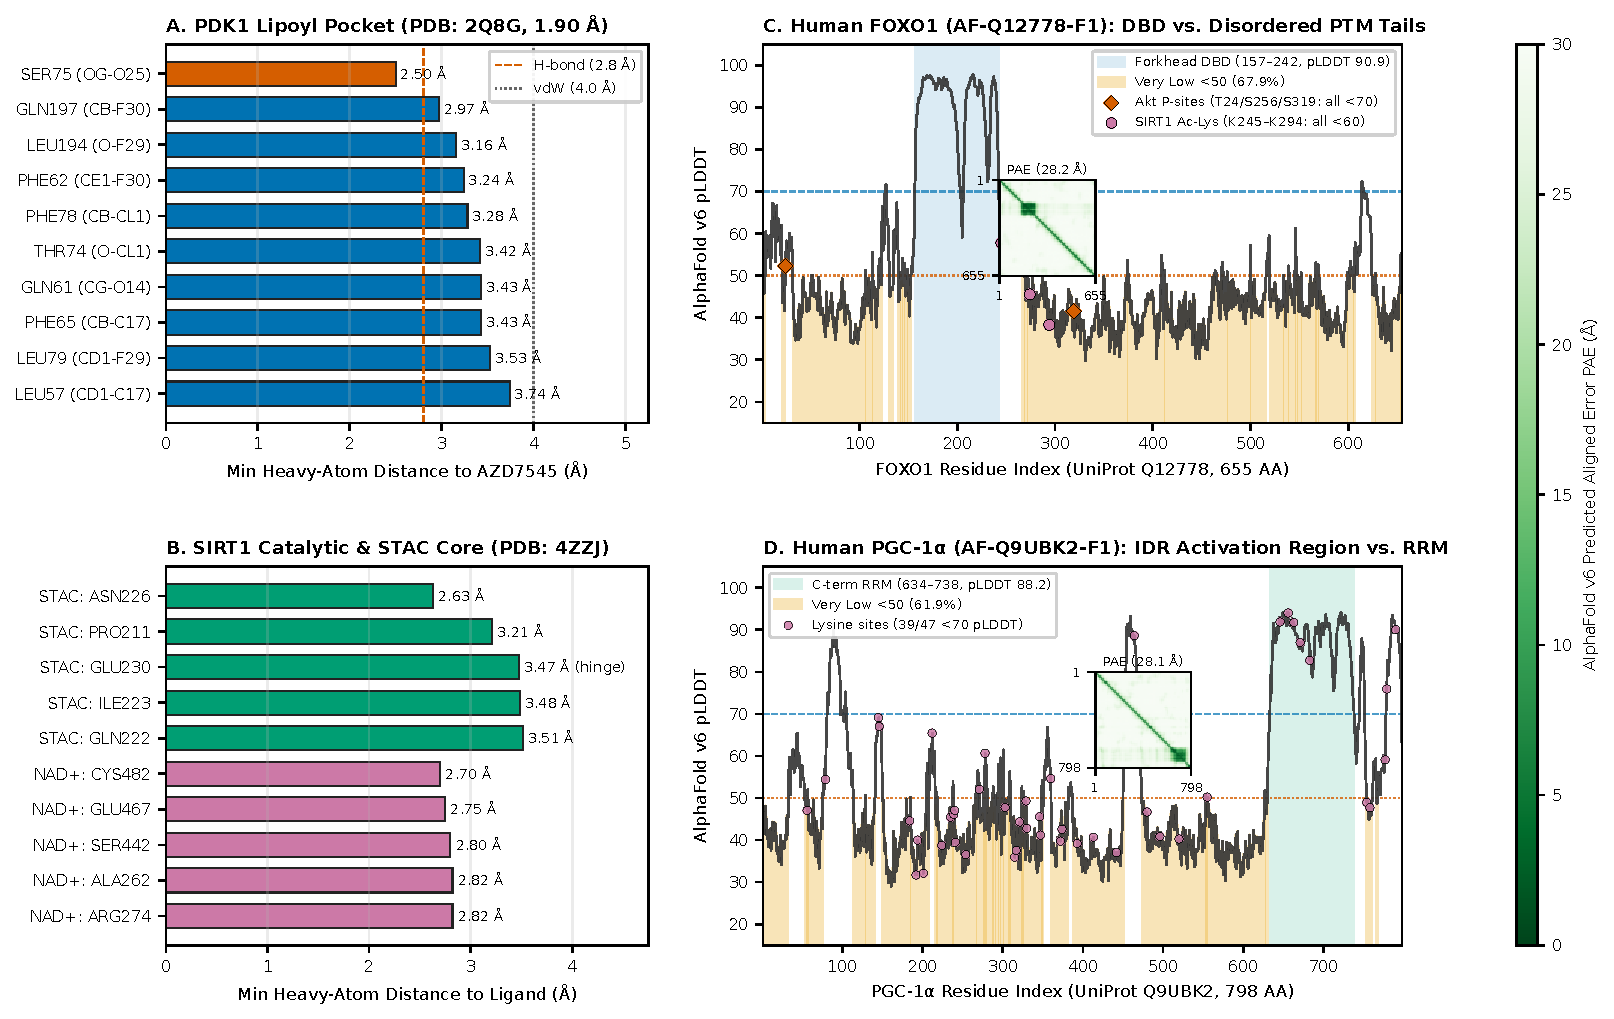
\includegraphics[width=\textwidth]{../../figures/paper2_fig1_structural_pharmacology_and_pae.pdf}
  \caption{\textbf{Atomic Ligand-Contact and AlphaFold v6 \texttt{pLDDT}/\texttt{PAE} Structural Bioinformatics Analysis Guiding Stage-2 Actuator Selection.} \textbf{(A)} Heavy-atom contacts ($\le 4.0\text{ \AA}$) between human \texttt{PDK1} and the allosteric inhibitor \texttt{AZD7545} (\texttt{AZX}) in \texttt{PDB: 2Q8G} ($1.90\text{ \AA}$ X-ray \cite{kato2007pdk1}), anchored by a $2.50\text{ \AA}$ hydrogen bond at \texttt{Ser75} ($\text{O}\gamma\text{--O25}$) inside the N-terminal lipoyl-binding (\texttt{L2}) pocket. \textbf{(B)} Heavy-atom contacts ($\le 4.0\text{ \AA}$) in human \texttt{SIRT1} (\texttt{PDB: 4ZZJ}, $2.74\text{ \AA}$ X-ray \cite{dai2015sirt1}) to the Sirtuin-Activating Compound \texttt{4TQ} (\texttt{Asn226} $2.63\text{ \AA}$; allosteric hinge \texttt{Glu230} $3.47\text{ \AA}$) and active-site carba-$\text{NAD}^+$ (\texttt{CNA}). \textbf{(C)} Full-length human \texttt{FOXO1} (\texttt{AF-Q12778-F1-v6}, $655\text{ AA}$): only the Forkhead DNA-binding domain (\texttt{residues 157--243}, mean $\mathrm{pLDDT} = 90.62$) is structured, whereas $9/9$ \texttt{Akt} phosphorylation (\texttt{Thr24, Ser256, Ser319}) and \texttt{SIRT1} deacetylation (\texttt{Lys245--Lys294}) sites reside in disordered segments ($\mathrm{pLDDT} < 70$; inset: $655 \times 655$ \texttt{PAE} matrix, off-diagonal mean $28.23\text{ \AA}$). \textbf{(D)} Full-length human \texttt{PGC-1$\alpha$} (\texttt{AF-Q9UBK2-F1-v6}, $798\text{ AA}$): only the C-terminal RNA-recognition motif (\texttt{residues 634--738}, mean $\mathrm{pLDDT} = 88.22$) is structured, whereas $39/47$ ($82.98\%$) of lysine residues and the entire N-terminal/central activation region (\texttt{1--633}) are disordered ($\mathrm{pLDDT} < 70$).}
  \label{fig:structural}
\end{figure*}

A central design question for Stage-2 metabolic consolidation is why pharmacological actuation must target upstream metabolic kinases and deacetylases (\texttt{PDK1} and \texttt{SIRT1}/$\text{NAD}^+$) rather than attempting direct small-molecule pocket activation of the master stemness transcription factors \texttt{FOXO1} and \texttt{PGC-1$\alpha$}. To ground our actuator parameterization in atomic coordinates, we audited experimental macromolecular crystallographic information files (\texttt{.cif}) from the Protein Data Bank alongside full-length AlphaFold Database v6 models and $N \times N$ Predicted Aligned Error (\texttt{PAE}) matrices \cite{jumper2021alphafold,varadi2024afdb} (Figure~\ref{fig:structural}, Table~\ref{tab:structural}).

\subsection{Druggable Allosteric Pockets in \texttt{PDK1} (\texttt{2Q8G}) and \texttt{SIRT1} (\texttt{4ZZJ})}
Coordinate inspection of human \texttt{PDK1} co-crystallized with the trifluoropropanamide inhibitor \texttt{AZD7545} (\texttt{PDB: 2Q8G}, Chain~A, $368$ resolved residues spanning \texttt{41--423} at $1.90\text{ \AA}$ resolution \cite{kato2007pdk1}) confirms that \texttt{AZD7545} (\texttt{AZX}, 31 heavy atoms) occupies the hydrophobic N-terminal lipoyl-binding (\texttt{L2}) pocket rather than the C-terminal ATP-binding cleft. Twelve residues form heavy-atom contacts $\le 4.0\text{ \AA}$ to \texttt{AZD7545} (Figure~\ref{fig:structural}A): a short $2.50\text{ \AA}$ hydrogen bond between \texttt{Ser75} ($\text{O}\gamma$) and the ligand hydroxyl ($\text{O25}$), flanked by \texttt{Gln197} ($2.97\text{ \AA}$), \texttt{Leu194} ($3.16\text{ \AA}$), \texttt{Phe62} ($3.24\text{ \AA}$), \texttt{Phe78} ($3.28\text{ \AA}$), \texttt{Thr74} ($3.42\text{ \AA}$), \texttt{Gln61} ($3.43\text{ \AA}$), \texttt{Phe65} ($3.43\text{ \AA}$), \texttt{Leu79} ($3.53\text{ \AA}$), \texttt{Leu57} ($3.74\text{ \AA}$), \texttt{Asp64} ($3.92\text{ \AA}$), and \texttt{Leu201} ($3.92\text{ \AA}$). By severing \texttt{PDK1} tethering to the dihydrolipoamide acetyltransferase (\texttt{E2}) core of the \texttt{PDH} complex, \texttt{AZD7545} unblocks pyruvate oxidation without competing against millimolar intramitochondrial ATP.

Similarly, coordinate audit of the engineered human \texttt{SIRT1} construct bound to Sirtuin-Activating Compound \texttt{4TQ} and active-site carba-$\text{NAD}^+$ (\texttt{PDB: 4ZZJ}, Chain~A, $344$ resolved residues within \texttt{183--660} at $2.74\text{ \AA}$ resolution \cite{dai2015sirt1}) resolves two distinct structured binding sites (Figure~\ref{fig:structural}B): (i) the N-terminal three-helix STAC-binding domain, where \texttt{4TQ} (36 heavy atoms) contacts \texttt{Asn226} ($2.63\text{ \AA}$ $\text{N}\delta2\text{--OAN}$ hydrogen bond), \texttt{Pro211} ($3.21\text{ \AA}$), the critical electrostatic hinge residue \texttt{Glu230} ($3.47\text{ \AA}$ $\text{O}\varepsilon1\text{--NAB}$), \texttt{Ile223} ($3.48\text{ \AA}$), and \texttt{Gln222} ($3.51\text{ \AA}$); and (ii) the Rossmann-fold $\text{NAD}^+$-binding pocket, where carba-$\text{NAD}^+$ (\texttt{CNA}, 44 heavy atoms) is coordinated by \texttt{Cys482} ($2.70\text{ \AA}$), \texttt{Glu467} ($2.75\text{ \AA}$), \texttt{Ser442} ($2.80\text{ \AA}$), \texttt{Ala262} ($2.82\text{ \AA}$), and \texttt{Arg274} ($2.82\text{ \AA}$).

\textbf{Chemical-Probe Caveat for \texttt{SIRT1} STACs:} Early synthetic STACs such as \texttt{SRT1720} were shown by Pacholec et al.~\cite{pacholec2010sirt1} to exhibit fluorophore-dependent artifacts on TAMRA-labeled peptides and off-target pharmacology in biochemical panels, while Hubbard et al.~\cite{hubbard2013sirt1} demonstrated that \texttt{Glu230}-mediated allosteric activation of native substrates requires bulky hydrophobic residues at positions $+1/+6$ C-terminal to the target acetyl-lysine. Consequently, in our model and postulated benchtop falsification protocol (\S\ref{sec:blueprint}), Stage-2 \texttt{SIRT1} activation ($u_{\mathrm{sirt}}$) primarily represents $\text{NAD}^+$ substrate repletion via nicotinamide riboside (\texttt{NR}, acting directly at the \texttt{Cys482}/\texttt{Glu467}/\texttt{Arg274} Rossmann pocket), with synthetic STACs treated strictly as an optional tool-compound arm requiring orthogonal genetic (\texttt{SIRT1} CRISPR knockout) and \texttt{Glu230Lys} point-mutant controls.

\subsection{Domain Architecture and PTM-Tail Disorder of \texttt{FOXO1} and \texorpdfstring{\texttt{PGC-1$\alpha$}}{PGC-1a}}
Full-length AlphaFold v6 structural audit reveals a sharp dichotomy between isolated nucleic-acid-binding domains and disordered post-translational modification (PTM) regions in both downstream effectors (Figure~\ref{fig:structural}C--D, Table~\ref{tab:structural}):
\begin{enumerate}
  \item \textbf{Human \texttt{FOXO1} (\texttt{AF-Q12778-F1-v6}, $655\text{ AA}$):} Global mean $\mathrm{pLDDT}$ is $50.96$, with $67.94\%$ ($445/655\text{ AA}$) in the \emph{Very Low} ($<50$) band, $18.17\%$ ($119/655$) in $50\text{--}70$, and $13.89\%$ ($91/655$) $\ge 70$, accompanied by a high off-diagonal mean $\mathrm{PAE} = 28.23\text{ \AA}$ ($1.86\%$ residue pairs $<5\text{ \AA}$). Contiguous domain segmentation ($\ge 25\text{ AA}$ with $\mathrm{pLDDT} \ge 70$) identifies \emph{one} structured domain: the winged-helix Forkhead DNA-binding domain (\texttt{residues 157--243}, $87\text{ AA}$, mean $\mathrm{pLDDT} = 90.62$, internal $\mathrm{PAE} = 4.70\text{ \AA}$). Crucially, however, \textbf{all 9/9 canonical regulatory PTM residues} controlling nuclear-cytoplasmic shuttling lie outside rigid tertiary pockets ($\mathrm{pLDDT} < 70$): the three \texttt{Akt} 14-3-3 phosphosites (\texttt{Thr24}: $52.28$, \texttt{Ser256}: $66.75$, \texttt{Ser319}: $41.56$) and all six \texttt{CBP/p300}/\texttt{SIRT1} acetyl-lysines (\texttt{Lys245}: $57.78$, \texttt{Lys248}: $53.19$, \texttt{Lys262}: $55.19$, \texttt{Lys265}: $52.41$, \texttt{Lys274}: $45.56$, \texttt{Lys294}: $38.28$).
  \item \textbf{Human \texttt{PGC-1$\alpha$} (\texttt{AF-Q9UBK2-F1-v6}, $798\text{ AA}$):} Global mean $\mathrm{pLDDT}$ is $52.74$ ($61.90\% < 50$, $17.17\%$ in $50\text{--}70$, $20.93\% \ge 70$; off-diagonal mean $\mathrm{PAE} = 28.12\text{ \AA}$, $1.26\%$ pairs $<5\text{ \AA}$). Segmentation detects \emph{one} structured C-terminal RNA-recognition motif (\texttt{RRM}, \texttt{residues 634--738}, $105\text{ AA}$, mean $\mathrm{pLDDT} = 88.22$, internal $\mathrm{PAE} = 7.79\text{ \AA}$), whereas the entire $633$-residue N-terminal and central transcriptional coactivation region---and $39/47$ ($82.98\%$) of all lysine residues across the protein (mean lysine $\mathrm{pLDDT} = 53.53$)---is intrinsically disordered.
\end{enumerate}
Rather than claiming that disordered transcription factors are universally ``undruggable,'' this structural audit explains \emph{mechanistically} why conventional pocket-based small-molecule discovery lacks preformed allosteric cavities in the PTM control regions of \texttt{FOXO1} and \texttt{PGC-1$\alpha$}, whereas the structured catalytic cleft of \texttt{SIRT1} (\texttt{PDB: 4ZZJ}) is evolutionarily specialized to capture flexible acetyl-lysine peptide motifs.

\begin{table*}[t]
\centering
\caption{\textbf{Verified Atomic-Coordinate and AlphaFold v6 Structural Bioinformatics Summary.} All metrics are computed directly from local \texttt{mmCIF} and \texttt{PAE} JSON coordinate files by \texttt{audit\_all\_structures()} in \texttt{simulator/generate\_paper2\_verified\_benchmarks.py}.}
\label{tab:structural}
\footnotesize
\resizebox{\textwidth}{!}{%
\begin{tabular}{@{}llllll@{}}
\toprule
\textbf{Target Protein} & \textbf{Structure / Accession} & \textbf{Length / Res.} & \textbf{Structured Domain(s)} & \textbf{Disorder / PAE Metrics} & \textbf{Verified Key Contacts or PTM Sites} \\
\midrule
\texttt{PDK1} (Kinase) & \texttt{PDB: 2Q8G} (X-ray) & $368\text{ AA}$ ($1.90\text{ \AA}$) & Lipoyl (\texttt{L2}) + Kinase core & Rigid co-crystal (\texttt{41--423}) & \texttt{AZD7545}: \texttt{Ser75} ($2.50\text{ \AA}$), \texttt{Gln197} ($2.97\text{ \AA}$), \texttt{Leu194} ($3.16\text{ \AA}$) \\
\texttt{SIRT1} (Deacetylase) & \texttt{PDB: 4ZZJ} (X-ray) & $344\text{ AA}$ ($2.74\text{ \AA}$) & STAC 3-helix + Rossmann & Rigid co-crystal (\texttt{183--660}) & \texttt{4TQ}: \texttt{Asn226} ($2.63\text{ \AA}$), \texttt{Glu230} ($3.47\text{ \AA}$); \texttt{CNA}: \texttt{Cys482} ($2.70\text{ \AA}$) \\
\texttt{FOXO1} (TF) & \texttt{AF-Q12778-F1-v6} & $655\text{ AA}$ (AF v6) & Forkhead DBD \texttt{157--243} ($90.6$) & $67.9\% <50$; $\mathrm{PAE}=28.23\text{ \AA}$ & $9/9$ \texttt{Akt} (\texttt{T24/S256/S319}) \& \texttt{Ac-Lys} (\texttt{K245--K294}) $<70$ $\mathrm{pLDDT}$ \\
\texttt{PGC-1$\alpha$} (Coact.) & \texttt{AF-Q9UBK2-F1-v6} & $798\text{ AA}$ (AF v6) & C-term RRM \texttt{634--738} ($88.2$) & $61.9\% <50$; $\mathrm{PAE}=28.12\text{ \AA}$ & \texttt{1--633} activation IDR; $39/47$ ($83.0\%$) lysines $<70$ $\mathrm{pLDDT}$ \\
\bottomrule
\end{tabular}%
}
\end{table*}

% =============================================================================
\section{In Silico Protocol Sweep, Target Ablations, and Adjoint Pareto Optimality}
\label{sec:optimal}
% =============================================================================

\begin{figure*}[t]
  \centering
  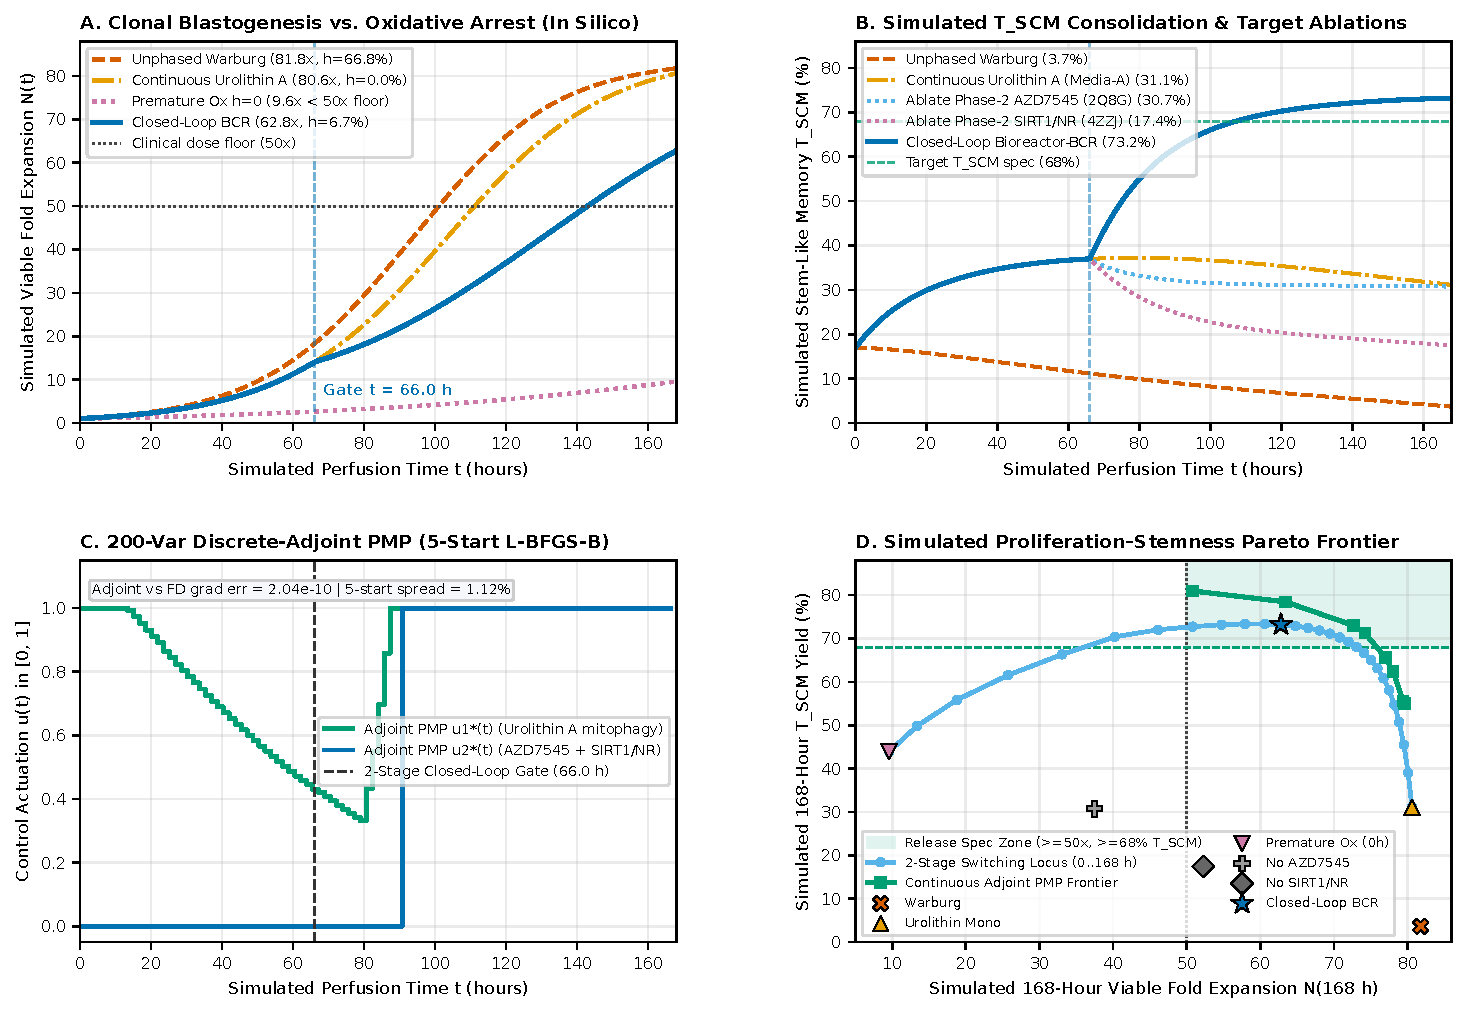
\includegraphics[width=\textwidth]{../../figures/paper2_fig2_bioreactor_ode_and_pareto_optimal.pdf}
  \caption{\textbf{\textit{In Silico} 168-Hour Perfusion Trajectories, Component Ablations, and 200-Variable Discrete-Adjoint Pareto Frontier.} \textbf{(A)} Simulated clonal fold expansion $N_{\mathrm{cells}}(t)$ showing Warburg glycolytic expansion ($81.77\times$, $h = 66.76\%$), premature Day-0 oxidative forcing ($9.58\times < 50\times$ clinical floor), continuous urolithin~A monotherapy ($80.60\times$), and closed-loop \textbf{Bioreactor-BCR} switching at $t_{\mathrm{gate}} = 66.02\text{ h}$ ($62.80\times$, $h = 6.73\%$). \textbf{(B)} Simulated $\mathrm{T}_{\mathrm{SCM}}(t)$ consolidation comparing closed-loop gating ($73.20\%$) against continuous urolithin~A without Stage-2 oxidative consolidation ($31.10\%$) and single-target Stage-2 ablations of \texttt{AZD7545} ($30.72\%$) or \texttt{SIRT1}/\texttt{NR} ($17.45\%$). \textbf{(C)} Unconstrained 200-variable discrete-adjoint Pontryagin optimal control schedule ($u_1^*(t), u_2^*(t)$ across $100$ intervals; maximum adjoint vs.\ central finite-difference gradient error across all $200$ variables $2.04 \times 10^{-10}$, 5-start \texttt{L-BFGS-B} objective spread $1.12\%$). \textbf{(D)} Simulated proliferation--stemness Pareto frontier comparing continuous PMP modulation against the 2-stage switching locus ($t_{\mathrm{sw}} \in [0, 168\text{ h}]$) and discrete baseline/ablation protocols.}
  \label{fig:pareto}
\end{figure*}

\subsection{Nominal Switching Sweep and Mechanistic Component Ablations}
To evaluate whether two-stage metabolic gating resolves the simulated proliferation--exhaustion conflict, we integrated the nominal 8-state system (\texttt{RK4}, $N = 1{,}000$ steps, $\Delta t = 0.168\text{ h}$) across 14 open-loop, closed-loop, and ablated regimens against five simultaneous manufacturing release criteria: viable expansion $N_{\mathrm{cells}}(168\text{ h}) \ge 50.0\times$, stemness $\mathrm{T}_{\mathrm{SCM}}(168\text{ h}) \ge 68.0\%$, exhaustion $E_{\mathrm{TOX}}(168\text{ h}) \le 15.0\%$, $\mathrm{SRC} \ge 3.5\times$, and depolarized organelle fraction $h(168\text{ h}) \le 10.0\%$ (Figure~\ref{fig:pareto}A--B, Table~\ref{tab:nominal}).

Unphased Warburg expansion ($u_1 = u_2 = 0$) achieves maximal cell yield ($81.77\times$) but drives severe mitochondrial depolarization ($h = 66.76\%$), supernatant lactatemia ($R_{\mathrm{LP}} = 30.02$, $\mathrm{pH} = 6.92$), nuclear \texttt{FOXO1} exclusion ($F_{\mathrm{nuc}} = 30.48\%$), $\text{TOX}^+$ commitment ($76.13\%$), and $\mathrm{T}_{\mathrm{SCM}}$ collapse ($3.67\%$). Conversely, premature oxidative switching at Hour~0 ($u_1 = 0, u_2 = 1$) stalls clonal division at $9.58\times$ ($<50\times$ floor) while failing to clear baseline depolarized mitochondria ($h = 64.81\%$). Continuous urolithin~A monotherapy ($u_1 = 1, u_2 = 0$, without Stage-2 galactose/\texttt{AZD7545}/\texttt{SIRT1} consolidation) thoroughly purges depolarized mitochondria ($h = 0.04\%$) and preserves blastogenesis ($80.60\times$), but because high glycolytic flux continues to drive Warburg exhaustion ($41.03\%$) and prevents full cristae $\mathrm{SRC}$ maturation ($2.26\times$), simulated $\mathrm{T}_{\mathrm{SCM}}$ plateaus at $31.10\%$.

Under nominal closed-loop gating ($h(t) \le 0.045$, $N_{\mathrm{cells}}(t) \ge 14.0\times$, $\mathrm{pH}(t) \ge 7.10$), \textbf{Bioreactor-BCR} transitions from Media-A to Media-B at $t_{\mathrm{gate}} = 66.02\text{ h}$ (accumulated selection integral $s(t_{\mathrm{gate}}) = 2.8248$), achieving $62.80\times$ fold expansion, $73.20\%$ $\mathrm{T}_{\mathrm{SCM}}$, $\mathrm{SRC} = 4.87\times$, $E_{\mathrm{TOX}} = 11.75\%$, and $h(168\text{ h}) = 6.73\%$---satisfying all five release criteria simultaneously. Ablating Stage-2 \texttt{AZD7545} ($u_{\mathrm{azd}} = 0$ after $66.02\text{ h}$) leaves \texttt{PDH} phosphorylated ($g_{\mathrm{pdh}} = 0.15$), cutting expansion in galactose-shifted media to $37.47\times$ and $\mathrm{T}_{\mathrm{SCM}}$ to $30.72\%$. Ablating Stage-2 \texttt{SIRT1}/\texttt{NR} activation ($u_{\mathrm{sirt}} = 0$ after $66.02\text{ h}$) allows $D$ to out-replicate $W$ ($k_{\mathrm{rep,adv}} = 1.22$), causing $h$ to rebound from $4.50\%$ at the gate to $36.27\%$ at $168\text{ h}$ and collapsing $\mathrm{T}_{\mathrm{SCM}}$ to $17.45\%$.

\begin{table*}[t]
\centering
\caption{\textbf{Nominal 168-Hour \textit{In Silico} Protocol Sweep, Target Ablations, and Discrete-Adjoint PMP Benchmark.} Release specification: $N \ge 50\times$, $\mathrm{T}_{\mathrm{SCM}} \ge 68\%$, $\mathrm{TOX}^+ \le 15\%$, $\mathrm{SRC} \ge 3.5\times$, and $h \le 10\%$.}
\label{tab:nominal}
\footnotesize
\resizebox{\textwidth}{!}{%
\begin{tabular}{@{}lcccccccc@{}}
\toprule
\textbf{Simulated Regimen} & $t_{\mathrm{gate}}$ (h) & $s(t_{\mathrm{gate}})$ & \textbf{Fold} $N(168\text{ h})$ & $\mathrm{T}_{\mathrm{SCM}}$ (\%) & $\mathrm{TOX}^+$ (\%) & $\mathrm{SRC}$ ($\times$) & $h(168\text{ h})$ (\%) & \textbf{5-Spec Pass} \\
\midrule
Unphased Warburg ($u_1=0, u_2=0$) & -- & -- & $81.77\times$ & $3.67\%$ & $76.13\%$ & $0.69\times$ & $66.76\%$ & Fail ($4/5$) \\
Premature Oxidative ($u_1=0, u_2=1$ from $0\text{ h}$) & $0.00$ & $0.0000$ & $9.58\times$ & $43.92\%$ & $27.64\%$ & $1.22\times$ & $64.81\%$ & Fail ($5/5$) \\
Continuous Urolithin~A Monotherapy ($u_1=1, u_2=0$) & -- & -- & $80.60\times$ & $31.10\%$ & $41.03\%$ & $2.26\times$ & $0.04\%$ & Fail ($3/5$) \\
Fixed Early Switch ($t_{\mathrm{sw}} = 36\text{ h}$) & $36.12$ & $1.4696$ & $46.11\times$ & $72.02\%$ & $9.32\%$ & $3.58\times$ & $23.51\%$ & Fail ($N, h$) \\
Fixed Intermediate Switch ($t_{\mathrm{sw}} = 48\text{ h}$) & $48.05$ & $2.0009$ & $54.72\times$ & $73.17\%$ & $10.16\%$ & $4.23\times$ & $14.87\%$ & Fail ($h > 10\%$) \\
\textbf{Closed-Loop Bioreactor-BCR} ($h \le 4.5\%$) & \textbf{66.02} & \textbf{2.8248} & \textbf{62.80}$\times$ & \textbf{73.20\%} & \textbf{11.75\%} & \textbf{4.87}$\times$ & \textbf{6.73\%} & \textbf{PASS ($5/5$)} \\
Fixed Late Switch ($t_{\mathrm{sw}} = 96\text{ h}$) & $96.10$ & $4.2392$ & $70.77\times$ & $70.26\%$ & $15.77\%$ & $5.13\times$ & $1.54\%$ & Fail ($\mathrm{TOX}^+$) \\
Fixed Very Late Switch ($t_{\mathrm{sw}} = 120\text{ h}$) & $120.12$ & $5.3857$ & $75.04\times$ & $65.03\%$ & $21.08\%$ & $4.78\times$ & $0.46\%$ & Fail ($\mathrm{T}_{\mathrm{SCM}}, \mathrm{TOX}^+$) \\
Ablate Stage-2 \texttt{AZD7545} (\texttt{PDB: 2Q8G}, $u_{\mathrm{azd}}=0$) & $66.02$ & $2.8248$ & $37.47\times$ & $30.72\%$ & $21.25\%$ & $2.66\times$ & $10.82\%$ & Fail ($5/5$) \\
Ablate Stage-2 \texttt{SIRT1}/\texttt{NR} (\texttt{PDB: 4ZZJ}, $u_{\mathrm{sirt}}=0$) & $66.02$ & $2.8248$ & $52.25\times$ & $17.45\%$ & $28.46\%$ & $1.62\times$ & $36.27\%$ & Fail ($4/5$) \\
\textbf{Discrete-Adjoint PMP Optimal} ($200\text{ vars}$, $\alpha=0.58$) & Cont. & -- & \textbf{71.15}$\times$ & \textbf{74.46\%} & \textbf{14.08\%} & \textbf{5.33}$\times$ & \textbf{0.09\%} & \textbf{PASS ($5/5$)} \\
\bottomrule
\end{tabular}%
}
\end{table*}

\subsection{200-Variable Discrete-Adjoint Optimal Control and Pareto Frontier}
To test whether a simple two-stage pinch-valve switch sacrifices substantial performance relative to an unconstrained, continuously modulated multi-pump schedule $(u_1(t), u_2(t)) \in [0, 1]^2$, we discretized $[0, 168\text{ h}]$ into $N_{\mathrm{ocp}} = 100$ piecewise-constant control intervals ($200$ decision variables) and minimized the exact scalarized terminal-plus-effort Bolza objective implemented in \texttt{solve\_discrete\_adjoint\_pareto()}:
\begin{align}
  J_\alpha(\mathbf{u}) &= -\alpha\frac{\mathrm{T}_{\mathrm{SCM}}(\mathbf{x}(T))}{100} - (1 - \alpha)\frac{N_{\mathrm{cells}}(\mathbf{x}(T))}{75.0} \nonumber\\
  &\quad + 0.45\Big(\frac{h(T)}{0.10}\Big)^2 + 0.35\,E_{\mathrm{TOX}}(T)^2 \nonumber\\
  &\quad + 2.50\Big(\frac{\max_\epsilon(0,\, 50.0 - N_{\mathrm{cells}}(T))}{50.0}\Big)^2 \nonumber\\
  &\quad + \frac{0.008}{N_{\mathrm{ocp}}}\sum_{k=0}^{N_{\mathrm{ocp}}-1}\big(u_{1,k}^2 + u_{2,k}^2\big),
  \label{eq:bolza}
\end{align}
where $\max_\epsilon(0, z) \equiv \frac{1}{2}(z + \sqrt{z^2 + \epsilon^2})$ ($\epsilon = 0.25$ on the $50\times$ dose floor; smooth hinge $\epsilon = 10^{-3}$ inside the differentiable discrete-adjoint ODE RHS, evaluated on the exact nonsmooth \texttt{RK4} plant at $N = 1{,}000$ fine steps for Table~\ref{tab:nominal}). Propagating exact discrete-time \texttt{RK4} stage-by-stage Jacobians backward via $\mathbf{p}_k = (\partial\Phi_k / \partial\mathbf{x}_k)^\top \mathbf{p}_{k+1}$ ($\mathbf{p}_k \in \mathbb{R}^8$) and verifying against central finite differences ($\epsilon_{\mathrm{FD}} = 10^{-6}$) across \emph{all $200$ decision variables} yields a maximum gradient discrepancy of $2.04 \times 10^{-10}$. Launching \texttt{L-BFGS-B} at the balanced Pareto weight $\alpha = 0.58$ from $5$ diverse initializations (two-stage step at $66.0\text{ h}$, uniform interior $u_1 = u_2 = 0.5$, early step at $36.0\text{ h}$, late step at $96.0\text{ h}$, and pseudo-random interior schedule $\mathcal{U}[0.1, 0.9]$) converges to a tight objective spread of $1.12\%$ ($J_{0.58}^* = -0.81366$ vs.\ two-stage closed-loop $J_{0.58} = -0.58290$, Table~\ref{tab:nominal}).

Interestingly, the Pontryagin-optimal control profile (Figure~\ref{fig:pareto}C) independently discovers a \emph{two-phase temporal structure}: it holds $u_2^*(t) = 0$ throughout Hours~$0\text{--}90.7$ while modulating $u_1^*(t)$ along a smooth interior arc ($1.0 \to 0.33$, avoiding the small $c_{\mathrm{akt}}$ glycolytic proliferation penalty once $h(t)$ is low), executes a brief $15\text{-hour}$ co-actuation overlap ($u_1^* = 1, u_2^* = 0 \to 1$) to block $k_{\mathrm{rep,adv}}$ rebound during initial mitochondrial biogenesis, and holds $u_1^* = u_2^* = 1$ to Hour~$168$. Sweeping $\alpha \in [0.08, 0.92]$ (Figure~\ref{fig:pareto}D) shows that while continuous multi-pump modulation expands yield from $62.80\times$ to $71.15\times$ ($+1.26\%$ $\mathrm{T}_{\mathrm{SCM}}$), the single-valve two-stage locus already enters well inside the 5-criteria clinical release zone without requiring continuous microfluidic drug mixing.

% =============================================================================
\section{Heterogeneous Oncology Cohort, Ratiometric \texttt{ORR} Observability, and Adaptive Extended-Horizon Rescue}
\label{sec:cohort}
% =============================================================================

\begin{figure*}[t]
  \centering
  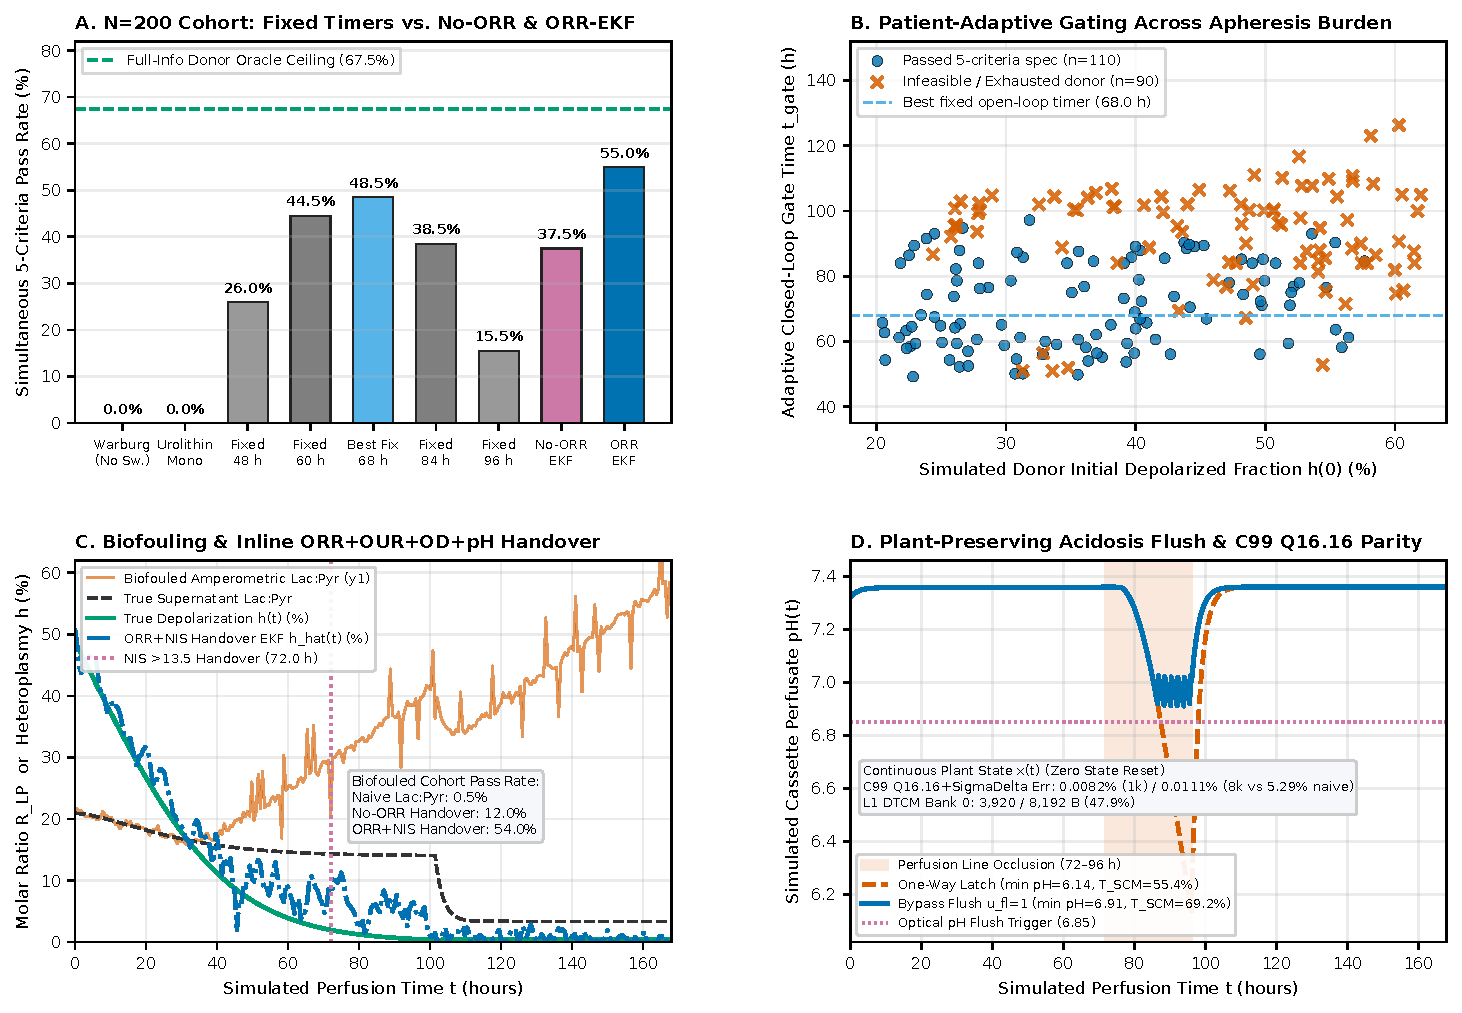
\includegraphics[width=\textwidth]{../../figures/paper2_fig3_donor_cohort_biofouling_and_acidosis.pdf}
  \caption{\textbf{$N = 1{,}000$ Heterogeneous Oncology Donor Cohort, Physical Volumetric \texttt{OUR}/\texttt{OD}/\texttt{ORR} Observability Under Biofouling, and Extended-Horizon Rescue.} \textbf{(A)} Simultaneous 5-criteria manufacturing pass rates across $N = 1{,}000$ simulated oncology apheresis donors comparing unphased baselines ($0.0\%$), open-loop fixed timers (peaking at $54.1\%$ at $68\text{ h}$), physical 4-channel EKF without \texttt{ORR} ($40.5\%$), 5-channel \texttt{ORR}-augmented Huber-EKF at $168\text{ h}$ ($58.7\%$; exact paired McNemar $p = 8.0 \times 10^{-4}$ vs.\ $68\text{ h}$, $p = 1.2 \times 10^{-41}$ vs.\ 4-channel), and \texttt{OD}-triggered adaptive harvest ($168\text{--}240\text{ h}$, $74.0\%$; $168\text{ h}$ oracle $74.3\%$, $240\text{ h}$ oracle $97.3\%$). \textbf{(B)} 2D oncology donor controllability phase space $(h_0, \mu_{\mathrm{glyc}}/\mu_{\mathrm{nom}})$ partitioning the $1{,}000$ donors into $168\text{ h}$ passers ($n = 587$), hypoproliferative donors rescued by $168\text{--}240\text{ h}$ adaptive harvest ($n = 169$), and unrescued severe-burden donors ($n = 244$). \textbf{(C)} Representative biofouling trajectory where enzymatic \texttt{Lac:Pyr} drift triggers $\mathrm{NIS} > 13.5$ residual handover at $67.8\text{ h}$ to the optical quartet (\texttt{OUR}$_{\mathrm{vol}}$+\texttt{OD}+\texttt{pH}+\texttt{ORR}), preserving a $59.4\%$ cohort pass rate ($p = 5.2 \times 10^{-129}$ vs.\ $12.3\%$ 4-channel handover). \textbf{(D)} Plant-preserving bypass neutral flush ($u_{\mathrm{fl}} = 1$, zero state reset) during perfusion-line occlusion ($72\text{--}96\text{ h}$), lifting $\min\mathrm{pH}$ from $6.14$ to $6.91$, alongside freestanding C99 \texttt{Q16.16} \texttt{RK4} ($0.0082\%$) and 5-channel EKF ($0.0216\%$) parity.}
  \label{fig:cohort}
\end{figure*}

\subsection{Volumetric Respirometry Bias vs.\ Cell-Density Cancellation in Ratiometric \texttt{ORR}}
In a physical closed-cassette perfusion bioreactor, inline dissolved-$\text{O}_2$ optodes do \emph{not} measure per-cell specific respiration directly; they measure \emph{volumetric} oxygen depletion proportional to total viable cell count $N_{\mathrm{cells}}$ times per-cell oxidative flux, while inline near-infrared (\texttt{NIR}) backscatter or capacitance probes estimate cell concentration subject to donor-specific lymphoblast-size calibration bias $\alpha_{\mathrm{OD}}$. To evaluate observability under realistic bioprocess physics and statistical power, we scaled our virtual cohort to $N = 1{,}000$ oncology apheresis donors ($h_0 \sim \mathcal{U}[0.20, 0.62]$, $M_0 \sim \mathcal{U}[0.85, 1.12]$, $R_{\mathrm{LP},0} \sim \mathcal{U}[18, 28]$, $F_{\mathrm{nuc},0} \sim \mathcal{U}[0.22, 0.36]$, $S_{\mathrm{SRC},0} \sim \mathcal{U}[1.05, 1.50]$, $E_{\mathrm{TOX},0} \sim \mathcal{U}[0.05, 0.14]$) with unmodeled kinetic perturbations ($\mu_{\mathrm{glyc}} \times \mathcal{U}[0.66, 1.36]$, $\mu_{\mathrm{ox}} \times \mathcal{U}[0.84, 1.16]$, $k_{\mathrm{mito},D,\max} \times \mathcal{U}[0.68, 1.36]$, $k_{\mathrm{Warburg}} \times \mathcal{U}[0.82, 1.22]$, $k_{\mathrm{warb,exh}} \times \mathcal{U}[0.82, 1.22]$) and unmodeled $\pm 6\%$ optical-density scattering bias $\alpha_{\mathrm{OD}} \sim \mathcal{U}[0.94, 1.06]$. The Huber-EKF runs strictly on \texttt{NOMINAL\_PARAMS} ($\hat{\alpha}_{\mathrm{OD}} = 1.00$) and never observes any donor's private parameters or initial state.

Sampled every $\Delta t_{\mathrm{obs}} = 0.30\text{ h}$ ($18\text{ min}$) under correlated $\mathrm{AR}(1)$ noise ($\rho = 0.65$), we compare:
\begin{enumerate}
  \item \textbf{Physical 4-Channel Cassette Suite (No \texttt{ORR}):} Amperometric supernatant ratio $y_1 = R_{\mathrm{LP}} + \nu_1$ ($\sigma_1 = 0.55$), \emph{volumetric} optode oxygen uptake $y_2 = \mathrm{OUR}_{\mathrm{vol}}(\mathbf{x}, u_2) + \nu_2 = N_{\mathrm{cells}}\,\mathrm{ATP}_{\mathrm{ox}}(\mathbf{x}, u_2) + \nu_2$ (heteroscedastic $\sigma_{2,k} = 0.030\sqrt{1 + (0.08 N_{\mathrm{cells}})^2}$), uncalibrated NIR optical density $y_3 = \alpha_{\mathrm{OD}} N_{\mathrm{cells}} + \nu_3$ ($\sigma_{3,k} = \sqrt{0.35^2 + (0.025 N_{\mathrm{cells}})^2}$), and phenol-red optical transmission $y_4 = \mathrm{pH} + \nu_4$ ($\sigma_4 = 0.018$).
  \item \textbf{5-Channel Optical-Metabolic Suite (With Ratiometric \texttt{ORR}):} Appends quartz-window two-band $\mathrm{FAD}/(\mathrm{FAD} + \mathrm{NAD(P)H})$ autofluorescence \cite{walsh2021omi}. Because bulk suspension fluorescence in both spectral bands scales linearly with illuminated cell concentration ($I_{\mathrm{FAD}} = \beta_{\mathrm{opt}} N_{\mathrm{cells}} W$, $I_{\mathrm{NAD(P)H}} = \beta_{\mathrm{opt}} N_{\mathrm{cells}}[D + c_{\mathrm{glyc}} g_{\mathrm{glc}}(u_2)]$), the unknown factor $\beta_{\mathrm{opt}} N_{\mathrm{cells}}$ \emph{cancels identically} in the ratio:
  \begin{align}
    y_5 &= \frac{I_{\mathrm{FAD}}}{I_{\mathrm{FAD}} + I_{\mathrm{NAD(P)H}}} + \nu_5 \nonumber\\
        &= \frac{W}{W + D + c_{\mathrm{glyc}}\,g_{\mathrm{glc}}(u_2)} + \nu_5,
    \label{eq:orr}
  \end{align}
  with $\sigma_5 = 0.012$, nominal $c_{\mathrm{glyc}} = 0.35$, and $\pm 8\%$ unmodeled donor variation in $c_{\mathrm{glyc}}$.
\end{enumerate}

In contrast, dividing volumetric respiration $y_2$ by biased optical density $y_3$ yields $y_2 / y_3 \approx \alpha_{\mathrm{OD}}^{-1}(W + \eta_D D)(1 + \gamma_{\mathrm{pdh}}u_2)(1 + \gamma_{\mathrm{src}}(S_{\mathrm{SRC}}-1)_+)$, which couples only to the sum $W + \eta_D D$ and inherits the permanent $\alpha_{\mathrm{OD}}^{-1}$ lymphoblast-size bias. Across the six core gating states $[W, D, N_{\mathrm{cells}}, R_{\mathrm{LP}}, S_{\mathrm{SRC}}, \mathrm{pH}]$, the 64-hour empirical Observability Gramian reflects this physical bottleneck: without \texttt{ORR}, $\kappa(\mathcal{G}_{4\mathrm{ch}}) = 5.37 \times 10^5$ and degrades $13.4\times$ upon $R_{\mathrm{LP}}$ electrode fouling to $\kappa(\mathcal{G}_{3\mathrm{ch,foul}}) = 7.21 \times 10^6$ ($\sigma_{\min} = 1.34 \times 10^{-5}$), yielding $\hat{h}$ RMSE $= 6.48\%$ (unfouled) and $16.18\%$ (biofouled). Adding ratiometric \texttt{ORR}~\eqref{eq:orr} supplies an orthogonal sensitivity row independent of $N_{\mathrm{cells}}$ and $\alpha_{\mathrm{OD}}$, improving post-fouling Gramian conditioning $8.55\times$ ($\kappa = 8.43 \times 10^5$) and holding $\hat{h}$ RMSE to $2.08\%$ (unfouled) and $2.15\%$ (biofouled).

\subsection{Explicit Switching Law, Guard Ablation, and $N = 1{,}000$ Paired McNemar Benchmarks}
To ensure complete controller transparency between Python and C99, the closed-loop Stage-$1 \to 2$ transition requires $4$ consecutive frames ($1.2\text{ h}$ persistence quorum) with $y_4 \ge 7.10$ and satisfaction of either the primary reachability gate or an explicit late-glycolysis exhaustion guard:
\begin{align}
  \mathcal{C}_{\mathrm{switch}}(t) &= \big(\hat{h} \le 0.056 \wedge \hat{N}_{\mathrm{cells}} \ge N_{\mathrm{req}}(t, \hat{\mu}_{\mathrm{rel}})\big) \nonumber\\
  &\;\vee \underbrace{\big(t \ge 83\text{ h} \wedge \hat{h} \le 0.072 \wedge \hat{N}_{\mathrm{cells}} \ge N_{\mathrm{guard}}\big)}_{\text{Late-glycolysis }\mathrm{TOX}^+\text{ ceiling guard}},
  \label{eq:switch_law}
\end{align}
where $\hat{\mu}_{\mathrm{rel}}(t) = \mathrm{clip}\big(\ln(\hat{N}_{\mathrm{cells}}(t)/\hat{N}_{\mathrm{cells}}(24\text{ h})) / [0.044(t - 24)],\, 0.78,\, 1.22\big)$ for $t \ge 28\text{ h}$ ($1.0$ for $t < 28\text{ h}$), predicted Stage-2 expansion factor $M_{\mathrm{S2}}(t) = \exp\big(0.0122\sqrt{\hat{\mu}_{\mathrm{rel}}(t)}\,(T_{\mathrm{plan}} - t)_+\big)$, and $N_{\mathrm{req}}(t, \hat{\mu}_{\mathrm{rel}}) = \mathrm{clip}\big(N_{\mathrm{target}} / \max(1.05,\, 0.58 M_{\mathrm{S2}} + 0.42\min(M_{\mathrm{S2}}, 3.6)),\, 14.0,\, 42.0\big)$ ($T_{\mathrm{plan}} = 168\text{ h}$, $N_{\mathrm{target}} = 52.5\times$ to buffer $\pm 6\%$ \texttt{OD} bias above the true $50\times$ floor, $N_{\mathrm{guard}} = 18.0\times$).

Across all $N = 1{,}000$ oncology donors (Figure~\ref{fig:cohort}A, Table~\ref{tab:cohort}), unphased Warburg, premature Hour-0 oxidative switching, and continuous urolithin~A monotherapy achieve $0.0\%$ ($0/1{,}000$) 5-criteria pass rates. Among nine open-loop fixed timers ($24\text{--}120\text{ h}$), performance peaks sharply at $t_{\mathrm{sw}} = 68\text{ h}$ ($54.1\%$, $541/1{,}000$) and $76\text{ h}$ ($52.8\%$). Because Warburg-flux and \texttt{OD} biases corrupt $\hat{h}$ without \texttt{ORR}, the 4-channel Huber-EKF achieves only $40.5\%$ ($405/1{,}000$). The 5-channel \texttt{ORR} Huber-EKF raises the 168-hour pass rate to \textbf{$58.7\%$ ($587/1{,}000$)}, significantly outperforming both the retrospective-best $68\text{ h}$ fixed timer ($+4.6\%$, paired $95\%$ CI $[+1.97\%, +7.23\%]$, exact two-sided McNemar $p = 8.04 \times 10^{-4}$; $114$ discordant wins vs.\ $68$ losses) and the 4-channel No-\texttt{ORR} EKF ($+18.2\%$, $95\%$ CI $[+15.58\%, +20.82\%]$, $p = 1.19 \times 10^{-41}$; $197$ vs.\ $15$). Ablating the $t \ge 83.0\text{ h}$ exhaustion guard in~\eqref{eq:switch_law} drops the 5-channel pass rate from $58.7\%$ to $49.9\%$ ($-8.8\%$, $95\%$ CI $[-10.58\%, -7.02\%]$, $p = 1.47 \times 10^{-25}$), confirming that capping glycolytic dwell time is essential to prevent $\mathrm{TOX}^+ > 15\%$ in high-$h_0$ donors. Under $100\%$ amperometric \texttt{Lac:Pyr} biofouling ($t_{\mathrm{foul}} \sim \mathcal{U}[30, 48]\text{ h}$), naive \texttt{Lac:Pyr} gating collapses to $0.5\%$ ($5/1{,}000$) and 4-channel $\mathrm{NIS}$ handover yields $12.3\%$ ($123/1{,}000$), whereas 5-channel \texttt{ORR}+$\mathrm{NIS}$ handover ($\mathrm{NIS}_1 > 13.5$ for $3$ frames, $1{,}000/1{,}000$ handovers) preserves \textbf{$59.4\%$ ($594/1{,}000$)} ($+47.1\%$ vs.\ No-\texttt{ORR} handover, $p = 5.22 \times 10^{-129}$; $+5.3\%$ vs.\ unfouled $68\text{ h}$ fixed timer, $p = 1.81 \times 10^{-4}$).

\subsection{Direct Test of Extended-Horizon ($168\text{--}240\text{ h}$) Rescue for Hypoproliferative Donors}
Evaluating the full-information donor oracle at $168\text{ h}$ shows that $74.3\%$ ($743/1{,}000$) of the cohort is controllable within $7\text{ days}$, leaving $25.7\%$ ($257/1{,}000$) infeasible at fixed $168\text{ h}$ (median $h_0 = 51.19\%$, $\mu_{\mathrm{glyc}}/\mu_{\mathrm{nom}} = 0.773\times$ vs.\ $38.79\%$ and $1.059\times$ in controllable donors). Rather than leaving extended culture as an untested conjecture, we simulated an adaptive variable-harvest policy ($T_{\mathrm{plan}} = 240\text{ h}$, $N_{\mathrm{target}} = 53.5\times$, $N_{\mathrm{guard}} = 14.0\times$) that harvests at $168\text{ h}$ whenever $\hat{N}_{\mathrm{cells}}(168\text{ h}) \ge 53.5\times$ with $\ge 36\text{ h}$ Stage-2 consolidation, and otherwise continues Stage-2 perfusion up to $240\text{ h}$ until $\hat{N}_{\mathrm{cells}}(t) \ge 53.5\times$. Extending the horizon raises the full-information oracle ceiling from $74.3\%$ to \textbf{$97.3\%$ ($973/1{,}000$)}---proving that $89.5\%$ ($230/257$) of $168\text{ h}$-infeasible runs fail solely from division-time truncation, while only $2.7\%$ ($27/1{,}000$; median $h_0 = 57.14\%$, fast Warburg exhaustion $\mu_{\mathrm{glyc}}/\mu_{\mathrm{nom}} = 1.189\times$) are intrinsically refractory even at $240\text{ h}$. In closed loop, \texttt{OD}-guided adaptive harvest extends culture past $168\text{ h}$ in only $22.5\%$ of donors yet rescues $169$ previously failing hypoproliferative runs (green triangles in Figure~\ref{fig:cohort}B), lifting the closed-loop pass rate from $58.7\%$ to \textbf{$74.0\%$ ($740/1{,}000$)} ($+15.3\%$, $95\%$ CI $[+12.81\%, +17.79\%]$, exact McNemar $p = 2.08 \times 10^{-33}$).

\begin{table*}[t]
\centering
\caption{\textbf{Simulated $N = 1{,}000$ Heterogeneous Oncology Apheresis Cohort, Guard/Sensor Ablations, Biofouling Handover, and Extended-Horizon ($168\text{--}240\text{ h}$) Rescue.} Medians and interquartile ranges (IQR) across all $1{,}000$ donors (seed \texttt{20261111}).}
\label{tab:cohort}
\footnotesize
\resizebox{\textwidth}{!}{%
\begin{tabular}{@{}lccccccc@{}}
\toprule
\textbf{Cohort Control Policy ($N=1{,}000$ Donors)} & \textbf{Pass Rate} & \textbf{Fold $N$ Med [IQR]} & \textbf{$\mathrm{T}_{\mathrm{SCM}}$ Med [IQR]} & \textbf{$\mathrm{TOX}^+$ Med} & \textbf{$h_{\mathrm{end}}$ Med} & \textbf{$\hat{h}$ RMSE} & \textbf{Gate $t_{\mathrm{sw}}$ Med [IQR]} \\
\midrule
Unphased Warburg ($u_1=0, u_2=0$, $168\text{ h}$) & $0.0\%$ ($0/1000$) & $80.7\times$ [$74.6, 83.7$] & $4.1\%$ [$1.8, 6.7$] & $75.0\%$ & $63.7\%$ & -- & -- \\
Continuous Urolithin~A Monotherapy ($168\text{ h}$) & $0.0\%$ ($0/1000$) & $81.3\times$ [$72.2, 83.9$] & $30.5\%$ [$28.9, 32.1$] & $42.0\%$ & $0.03\%$ & -- & -- \\
Open-Loop Fixed Timer ($48\text{ h}$) & $24.7\%$ ($247/1000$) & $55.7\times$ [$42.1, 66.1$] & $72.9\%$ [$71.1, 74.2$] & $10.9\%$ & $13.1\%$ & -- & $48.0\text{ h}$ (fixed) \\
Open-Loop Fixed Timer ($60\text{ h}$) & $45.0\%$ ($450/1000$) & $61.8\times$ [$47.2, 71.6$] & $72.9\%$ [$71.5, 73.9$] & $11.9\%$ & $7.5\%$ & -- & $60.0\text{ h}$ (fixed) \\
\textbf{Best Open-Loop Fixed Timer ($68\text{ h}$)} & \textbf{54.1\%} ($541/1000$) & $64.9\times$ [$50.3, 74.3$] & $72.5\%$ [$71.3, 73.6$] & $12.7\%$ & $5.1\%$ & -- & $68.0\text{ h}$ (fixed) \\
Open-Loop Fixed Timer ($84\text{ h}$) & $42.2\%$ ($422/1000$) & $69.5\times$ [$55.0, 77.5$] & $71.2\%$ [$70.0, 72.2$] & $14.6\%$ & $2.3\%$ & -- & $84.0\text{ h}$ (fixed) \\
Open-Loop Fixed Timer ($96\text{ h}$) & $15.4\%$ ($154/1000$) & $72.1\times$ [$58.1, 79.2$] & $69.5\%$ [$68.3, 70.7$] & $16.5\%$ & $1.2\%$ & -- & $96.0\text{ h}$ (fixed) \\
Ablation: Physical 4-Ch EKF (\textbf{No \texttt{ORR}}, $168\text{ h}$) & $40.5\%$ ($405/1000$) & $68.9\times$ [$58.4, 75.8$] & $70.7\%$ [$66.2, 72.4$] & $14.9\%$ & $1.81\%$ & $6.48\%$ & $84.6\text{ h}$ [$66.5, 100.7$] \\
Ablation: 5-Ch \texttt{ORR} EKF (\textbf{No $83\text{ h}$ Guard}, $168\text{ h}$) & $49.9\%$ ($499/1000$) & $66.5\times$ [$58.4, 73.1$] & $71.1\%$ [$68.3, 72.7$] & $14.3\%$ & $3.81\%$ & $2.12\%$ & $79.4\text{ h}$ [$63.0, 102.3$] \\
\textbf{Closed-Loop 5-Ch \texttt{ORR} Huber-EKF ($168\text{ h}$)} & \textbf{58.7\%} ($587/1000$)$^{\dagger}$ & $66.4\times$ [$56.2, 73.1$] & $71.7\%$ [$70.2, 72.8$] & $13.7\%$ & $4.34\%$ & \textbf{2.08\%} & $79.4\text{ h}$ [$63.0, 90.6$] \\
Biofouled \texttt{Lac:Pyr}: Naive Threshold Gate & $0.5\%$ ($5/1000$) & $81.2\times$ [$72.2, 83.9$] & $30.5\%$ [$29.0, 32.1$] & $42.0\%$ & $0.03\%$ & $47.26\%$ & $50.7\text{ h}$ ($n=5$) \\
Biofouled \texttt{Lac:Pyr}: 4-Ch No-\texttt{ORR} $\mathrm{NIS}$ Handover & $12.3\%$ ($123/1000$) & $74.2\times$ [$62.6, 80.8$] & $65.2\%$ [$60.3, 69.0$] & $20.9\%$ & $0.57\%$ & $16.18\%$ & $115.8\text{ h}$ [$99.9, 129.9$] \\
\textbf{Biofouled \texttt{Lac:Pyr}: 5-Ch \texttt{ORR} + $\mathrm{NIS}$ Handover} & \textbf{59.4\%} ($594/1000$)$^{\ddagger}$ & $67.0\times$ [$56.0, 73.5$] & $71.6\%$ [$70.2, 72.8$] & $13.9\%$ & $3.99\%$ & \textbf{2.15\%} & $82.1\text{ h}$ [$64.5, 90.6$] \\
\textbf{Adaptive Horizon ($168\text{--}240\text{ h}$) 5-Ch \texttt{ORR} EKF} & \textbf{74.0\%} ($740/1000$)$^{\S}$ & $65.7\times$ [$55.3, 73.1$] & $72.4\%$ [$71.2, 73.4$] & $13.1\%$ & $4.87\%$ & \textbf{2.06\%} & $73.8\text{ h}$ [$62.0, 84.6$] \\
\midrule
Full-Information Donor Oracle Ceilings ($168\text{ h}$ / $240\text{ h}$) & \multicolumn{7}{l}{$74.3\%$ ($743/1000$) at fixed $168\text{ h}$;\quad $97.3\%$ ($973/1000$) with $168\text{--}240\text{ h}$ extended harvest ($2.7\%$ intrinsically refractory)} \\
\bottomrule
\multicolumn{8}{@{}l}{\scriptsize Exact two-sided paired McNemar tests: $^{\dagger}p = 8.04 \times 10^{-4}$ vs.\ $68\text{ h}$ fixed ($+4.6\%$), $p = 1.19 \times 10^{-41}$ vs.\ 4-Ch No-\texttt{ORR} ($+18.2\%$); $^{\ddagger}p = 5.22 \times 10^{-129}$ vs.\ 4-Ch handover; $^{\S}p = 2.08 \times 10^{-33}$ vs.\ $168\text{ h}$ EKF.}
\end{tabular}%
}
\end{table*}

% =============================================================================
\section{Plant-Preserving Acidosis Rescue and Deterministic Fixed-Point Safety Firmware}
\label{sec:hardware}
% =============================================================================

\subsection{Continuous-Plant Neutral Bypass Flush Under Perfusion Occlusion}
As established in Paper~I \cite{satz2026paper1}, restoring a microcontroller's internal estimator memory after a fault cannot reset biological state variables; actuator recovery must operate strictly through continuous plant dynamics $\mathbf{x}(t)$. In hollow-fiber CAR-T cassettes, a primary post-switch hazard is partial peristaltic line occlusion or gas-transfer fouling during high-density Stage-2 expansion ($N_{\mathrm{cells}} > 20\times$). We simulated a $24\text{-hour}$ Media-B perfusion-line occlusion across Hours~$72\text{--}96$ ($92\%$ drop in main-line exchange $k_{\mathrm{perf},0}$ and $k_{\mathrm{perf,LP}}$, loss of \texttt{AZD7545} delivery $u_{\mathrm{azd,eff}} = 0$, and hypoxic glycolytic surge $1.65\times k_{\mathrm{acid}}$, Figure~\ref{fig:cohort}D).

Under a one-way valve latch ($u_{\mathrm{fl}} = 0$), cassette perfusate $\mathrm{pH}(t)$ plunges to $\min\mathrm{pH} = 6.14$, triggering severe acidotic \texttt{FOXO1} nuclear export~\eqref{eq:ode_F} and $\text{TOX}^+$ commitment~\eqref{eq:ode_E} ($E_{\mathrm{TOX}} = 32.28\%$, $\mathrm{T}_{\mathrm{SCM}} = 55.39\%$). When the supervisory controller monitors optical phenol-red $\mathrm{pH}(t) \le 6.85$ and opens the auxiliary neutral-buffer bypass flush ($u_{\mathrm{fl}} = 1$, reverting to protective Stage-1 media for a $6\text{-hour}$ stabilization window without altering $\mathbf{x}(t)$ discontinuously), $\min\mathrm{pH}$ is arrested at $6.91$, limiting $E_{\mathrm{TOX}}$ to $16.11\%$ and rescuing simulated $\mathrm{T}_{\mathrm{SCM}}$ to $69.16\%$ ($N_{\mathrm{cells}} = 70.59\times$, $h = 8.14\%$).

\subsection{Freestanding FPU-Free C99 \texttt{RK4} and 5-Channel Huber-EKF Verification}
Unlike implantable neural devices or solar agricultural sensors, a benchtop GMP cell-therapy bioreactor is wall-powered; embedded microwatt sleep budgets are not a bioprocess bottleneck. Instead, regulatory software verification for single-use disposable cassette controllers (\texttt{IEC~62304} safety class) prioritizes \emph{deterministic execution without dynamic heap allocation (\texttt{malloc}), absence of non-deterministic floating-point library (\texttt{<math.h>}) or FPU exceptions, and statically bounded SRAM residency} portable to FPU-less safety microcontrollers and integer RISC-V cores (\texttt{RV32IM}/\texttt{Zve32x}). We therefore implemented the complete 8-state cassette plant, $\Sigma\Delta$ \texttt{RK4} predictor, 5-channel sequential Huber-EKF, integer $\mathrm{NIS}$ biofouling monitor, and acidosis bypass-flush state machine in freestanding integer C99 (\texttt{build/coralnpu/cart\_bioreactor\_hil\_testbench.c}, compiled under \texttt{-O2 -Wall -Wextra -Werror -std=c99} with zero unused neural-network weight tables).

States are stored in signed 32-bit \texttt{Q16.16} with dynamic pre-scaling ($N_{\mathrm{cells}}/64$, $R_{\mathrm{LP}}/32$, $S_{\mathrm{SRC}}/8$, $\mathrm{pH}/8$), \texttt{RK4} slopes in \texttt{Q8.24} ($2^{-24} \approx 5.96 \times 10^{-8}$) with 64-bit $\Sigma\Delta$ remainder tracking, and the $8 \times 8$ EKF covariance matrix $\mathbf{P}$ in signed \texttt{Q12.20} (spanning $[10^{-6}, 2048)$ so both initial $R_{\mathrm{LP}}$ variance $4.0$ and optical \texttt{ORR} noise variance $1.44 \times 10^{-4}$ are resolved without overflow or underflow). Sequential scalar measurement updates use an exact 64-bit integer square root (\texttt{isqrt64\_u32}) for Huber innovation clipping ($|\nu_i| \le 2.5\sqrt{S_i}$) and an exact division-free integer biofouling check ($2\nu_1^2 > 27 S_1 \iff \mathrm{NIS}_1 > 13.5$). Table~\ref{tab:hardware} summarizes exact metrics emitted by \texttt{cart\_bioreactor\_hil\_testbench.c -\/-json}:
\begin{enumerate}
  \item \textbf{Zero-Heap Static SRAM Footprint:} Removing unused neural projection weights shrinks \texttt{sizeof(coralnpu\_cart\_dtcm\_bank0\_workspace\_t)} to $2{,}704\text{ B}$ ($33.01\%$ of an $8{,}192\text{ B}$ SRAM bank), encompassing all \texttt{Q16.16} state/checkpoint vectors, \texttt{Q12.20} $8 \times 8$ covariance and process-noise matrices, \texttt{Q8.24} \texttt{RK4}/$\Sigma\Delta$ registers, 64-frame persistence buffers, and stack margin.
  \item \textbf{Deadband-Free \texttt{RK4} Parity Across Step Sizes:} At $N = 1{,}000$ steps, \texttt{Q16.16}+$\Sigma\Delta$ matches \texttt{FP64} switching time to the exact step ($66.024\text{ h}$), final expansion ($62.7802\times$ vs.\ $62.7979\times$), and $\mathrm{T}_{\mathrm{SCM}}$ ($73.1881\%$ vs.\ $73.1989\%$), keeping normalized $\ell_2$ trajectory error flat at \textbf{$0.0078\%\text{--}0.0114\%$} across $N \in \{500, \dots, 8{,}000\}$ ($478\times$ lower than naive \texttt{Q16.16}'s $5.2906\%$ drift at $N = 8{,}000$).
  \item \textbf{Full Integer 5-Channel Huber-EKF \& $\mathrm{NIS}$ Handover Parity:} Across $560$ closed-loop frames ($168\text{ h}$) on a mismatched, biofouled oncology donor ($h_0 = 51.0\%$, $\alpha_{\mathrm{OD}} = 1.05$), the integer C99 5-channel Huber-EKF achieves $\hat{h}$ RMSE $= 2.3389\%$ vs.\ $2.3346\%$ in IEEE-754 \texttt{FP64} (\textbf{$0.0216\%$ C99-vs.-\texttt{FP64} trajectory difference}), triggering $\mathrm{NIS}_1 > 13.5$ optical handover ($58.20\text{ h}$) and closed-loop switching ($84.00\text{ h}$) at the exact same frames as \texttt{FP64}.
\end{enumerate}

\begin{table}[t]
\centering
\caption{\textbf{Freestanding FPU-Free C99 Fixed-Point Plant and 5-Channel Huber-EKF Verification.} Exact metrics emitted directly by \texttt{cart\_bioreactor\_hil\_testbench.c -\/-json}.}
\label{tab:hardware}
\footnotesize
\resizebox{\columnwidth}{!}{%
\begin{tabular}{@{}lcc@{}}
\toprule
\textbf{Firmware / Numerical Verification Metric} & \textbf{IEEE-754 \texttt{FP64}} & \textbf{Integer C99 (\texttt{Q16.16}/\texttt{Q12.20}/\texttt{Q8.24})} \\
\midrule
Zero-Heap Static SRAM Workspace (\texttt{sizeof}) & -- & $2{,}704\text{ B} / 8{,}192\text{ B}$ ($33.01\%$) \\
Nominal Gate Switch Time ($N=1{,}000$) & $66.024\text{ h}$ & $66.024\text{ h}$ \\
Nominal Fold Expansion $N(168\text{ h})$ & $62.7979\times$ & $62.7802\times$ \\
Nominal $\mathrm{T}_{\mathrm{SCM}}(168\text{ h})$ / $h(168\text{ h})$ & $73.1989\%\;/\;6.7257\%$ & $73.1881\%\;/\;6.7253\%$ \\
\texttt{RK4} $\ell_2$ Error ($N = 500\;/\;1{,}000\;/\;2{,}000$) & Ref. & $0.0085\%\;/\;0.0082\%\;/\;0.0078\%$ \\
\texttt{RK4} $\ell_2$ Error ($N = 4{,}000\;/\;8{,}000$) & Ref. & $0.0114\%\;/\;0.0111\%$ \\
\textit{Naive \texttt{Q16.16} Error ($N = 1{,}000\;/\;8{,}000$)} & Ref. & \textit{$0.6412\%\;/\;5.2906\%$ (drift)} \\
5-Ch Huber-EKF $\hat{h}$ RMSE (Biofouled Run) & $2.3346\%$ & $2.3389\%$ ($0.0216\%$ diff) \\
$\mathrm{NIS} > 13.5$ Handover / Closed-Loop Gate & $58.20\text{ h}\;/\;84.00\text{ h}$ & $58.20\text{ h}\;/\;84.00\text{ h}$ \\
Acidosis Fault $\min\mathrm{pH}$ (No Flush / Flush) & $6.1366\;/\;6.9106$ & $6.1366\;/\;6.9106$ \\
\bottomrule
\end{tabular}%
}
\end{table}

% =============================================================================
\section{Limitations, Postulated Ex Vivo Falsification Blueprint, and Reproducibility}
\label{sec:blueprint}
% =============================================================================

\subsection{Model Limitations and Modeling Assumptions}
Several limitations bound the interpretation of these computational results:
\begin{enumerate}
  \item \textbf{Absence of Wet-Lab Execution:} No primary human T~cells, CAR lentiviral vectors, or bioreactor cassettes were experimentally cultured in this study. Rate constants tagged \textbf{[F]} in Table~\ref{tab:cart_params} represent phenomenologically calibrated couplings synthesized from separate immunological and structural reports \cite{fraietta2018determinants,doan2024foxo1,chan2024foxo1,denk2022immunity} rather than joint system-identification fits to a single time-series dataset.
  \item \textbf{Deterministic Population-Mean Approximation:} Equations~\eqref{eq:ode_W}--\eqref{eq:ode_pH} track mean intracellular organelle mass and population-level $\mathrm{T}_{\mathrm{SCM}}$/$\mathrm{TOX}^+$ fractions, neglecting clone-to-clone CAR copy-number variance, $\text{CD4}^+/\text{CD8}^+$ subset interactions, and asymmetric mitochondrial partitioning at cytokinesis.
  \item \textbf{Optical Redox Confounding at High Suspension Density:} While cell concentration cancels in first-order two-band autofluorescence \texttt{ORR}~\eqref{eq:orr} \cite{walsh2021omi}, inner-filter reabsorption at ultra-high hollow-fiber densities ($>3 \times 10^7\text{ cells/mL}$) and riboflavin/phenol-red media fluorescence require synchronized cell-free perfusate blanking in physical hardware.
\end{enumerate}

\subsection{Postulated Ex Vivo Benchtop Falsification Protocol}
To enable direct experimental falsification without requiring \textit{in vivo} animal studies, our simulations generate concrete, quantitative predictions testable in a 5-arm parallel perfusion bioreactor study using primary human $\text{CD19-BB}\zeta$ CAR-T cells from $n \ge 20$ pretreated oncology donor apheresis samples:
\begin{itemize}
  \item \textbf{Arm~1 (Standard Warburg Control):} $25\text{ mM}$ glucose + $300\text{ IU/mL}$ IL-2 ($0\text{--}168\text{ h}$). \textit{Prediction:} High expansion ($>70\times$), high $\text{TMRE}^{\mathrm{low}}/\text{MitoTracker}^{\mathrm{high}}$ depolarized fraction ($>50\%$), $\mathrm{T}_{\mathrm{SCM}} < 10\%$.
  \item \textbf{Arm~2 (Continuous Urolithin~A Monotherapy):} Media-A ($25\,\mu\mathrm{M}$ urolithin~A) continuously ($0\text{--}168\text{ h}$) in $25\text{ mM}$ glucose. \textit{Prediction:} Clearance of $\text{TMRE}^{\mathrm{low}}$ mitochondria ($<5\%$) but incomplete $\mathrm{T}_{\mathrm{SCM}}$ conversion ($\sim 25\text{--}35\%$) due to persistent glycolytic $\text{TOX}^+$ acquisition.
  \item \textbf{Arm~3 (Fixed $68\text{ h}$ Open-Loop Switch):} Media-A ($0\text{--}68\text{ h}$) switched blindly at $68.0\text{ h}$ to Media-B ($6.5\text{ mM}$ glucose + $18.5\text{ mM}$ galactose, $1.0\,\mu\mathrm{M}$ \texttt{AZD7545}, $1.0\text{ mM}$ nicotinamide riboside, $10\text{ ng/mL}$ IL-7/IL-15).
  \item \textbf{Arm~4 (Chemical-Probe-Free \texttt{ORR}-EKF Closed-Loop + Adaptive $168\text{--}240\text{ h}$ Harvest):} Closed-loop \texttt{ORR}+\texttt{OUR}$_{\mathrm{vol}}$+\texttt{OD}+\texttt{pH} Huber-EKF switching~\eqref{eq:switch_law} from Media-A to STAC-free Media-B (\texttt{AZD7545} + \texttt{NR} only, avoiding \texttt{SRT1720} off-target risk \cite{pacholec2010sirt1}), with \texttt{OD}-triggered harvest up to $240\text{ h}$ for slow-dividing donors. \textit{Falsification Criterion:} The model is falsified if Arm~4 fails to increase the 5-criteria pass rate ($N \ge 50\times$, $\text{CD45RA}^+\text{CD62L}^+\text{TCF7}^+ \ge 68\%$, $\mathrm{TOX}^+ \le 15\%$, Seahorse $\mathrm{SRC} \ge 3.5\times$) relative to Arm~3, or if hypoproliferative ($\mu_{\mathrm{glyc}} < 0.85\mu_{\mathrm{nom}}$) donors fail to reach $\ge 50\times$ viable fold expansion during the $168\text{--}240\text{ h}$ consolidation window (Figure~\ref{fig:cohort}B).
  \item \textbf{Arm~5 (\texttt{SIRT1}-KO / \texttt{Glu230Lys} \& Single-Target Ablation Controls):} Closed-loop switching omitting either \texttt{AZD7545} or \texttt{NR} (testing the single-target ablation collapse predicted in Table~\ref{tab:nominal}), plus \texttt{SIRT1} CRISPR knockout / \texttt{Glu230Lys} point-mutant specificity controls if synthetic STACs (\texttt{4TQ}/\texttt{SRT2104}) are evaluated \cite{hubbard2013sirt1}.
\end{itemize}

\subsection{Code and Reproducibility Availability (MIASE)}
All structural audits, 8-state \texttt{FP64} simulations, 200-variable discrete-adjoint \texttt{L-BFGS-B} optimizations, Observability Gramians, $N = 1{,}000$ donor Monte Carlo runs and exact paired McNemar tests (PRNG seed \texttt{20261111}), publication vector figures, and freestanding C99 fixed-point verification benchmarks are deterministically regenerated from source via \path{simulator/generate_paper2_verified_benchmarks.py} and \path{build/coralnpu/cart_bioreactor_hil_testbench.c} at \url{https://github.com/deesatzed/mitorestorer}.

\section*{Acknowledgments and Disclosures}
\footnotesize
\noindent\textbf{Acknowledgments \& Program Support:} This research was supported by Google LLC through the \textbf{Google AI for Science Researcher Access Program}, providing access to Google DeepMind's \textbf{Antigravity} agentic research environment, Gemini frontier reasoning models, and integrated structural biology and AlphaFold Database tools.\\
\noindent\textbf{Author Contributions \& AI Collaboration Disclosure:} This study was conceived, directed, and conducted solely by Wayne A.~Satz, MD in direct collaboration with Google DeepMind's Antigravity AI research agent; no other human investigators participated. Antigravity assisted with structural bioinformatics coordinate audits, mathematical derivation checks, Python discrete-adjoint and EKF cohort simulations, freestanding C99 fixed-point firmware implementation, and \LaTeX{} manuscript preparation. Wayne A.~Satz, MD audited, verified, and takes full scholarly responsibility for the integrity of all equations, code artifacts, numerical benchmarks, and scientific conclusions.\\
\noindent\textbf{Competing Interests:} The author declares no competing financial or commercial interests.\\
\noindent\textbf{Ethics Statement:} This study consists exclusively of theoretical modeling, structural bioinformatics on public Protein Data Bank / AlphaFold entries, numerical ODE simulation, and host-emulated firmware verification; no human participants, primary donor tissues, clinical cohorts, or live animals were involved.

\bibliographystyle{unsrt}
\bibliography{references}

\end{document}
